\newpage
\onecolumn
\begin{appendices}
    \section{SPICE Netlists}
    
    \begin{verbbox}
        \footnotesize\verb|pushpullphi2_new.sp|
    \end{verbbox}
    \lstinputlisting[language=spice,label=lst:spice-netlist,caption={{\verbBox} LTspice Netlist for converter simulation}] {listing/pushpullphi2_new.sp}
    %\section{Python Programs}
    %\lipsum[1]
    %\section{MATLAB Programs}
    %\lipsum[1]
    \centering
    \section{Physical Schematics, Bills of Materials, PCB Layouts, \& Assembled Boards}
    \label{sec:appendix:pcb}
    \begin{figure}[H]
        \centering
        \includestandalone[width=0.4\linewidth]{figure/tikz/PCB-Color-Map}
        \label{fig:pcb-color-map}
        \caption{Color code for PCB prints}
    \end{figure}
    \newpage
    \subsection{Inverter}
    \begin{figure}[H]
        \centering
        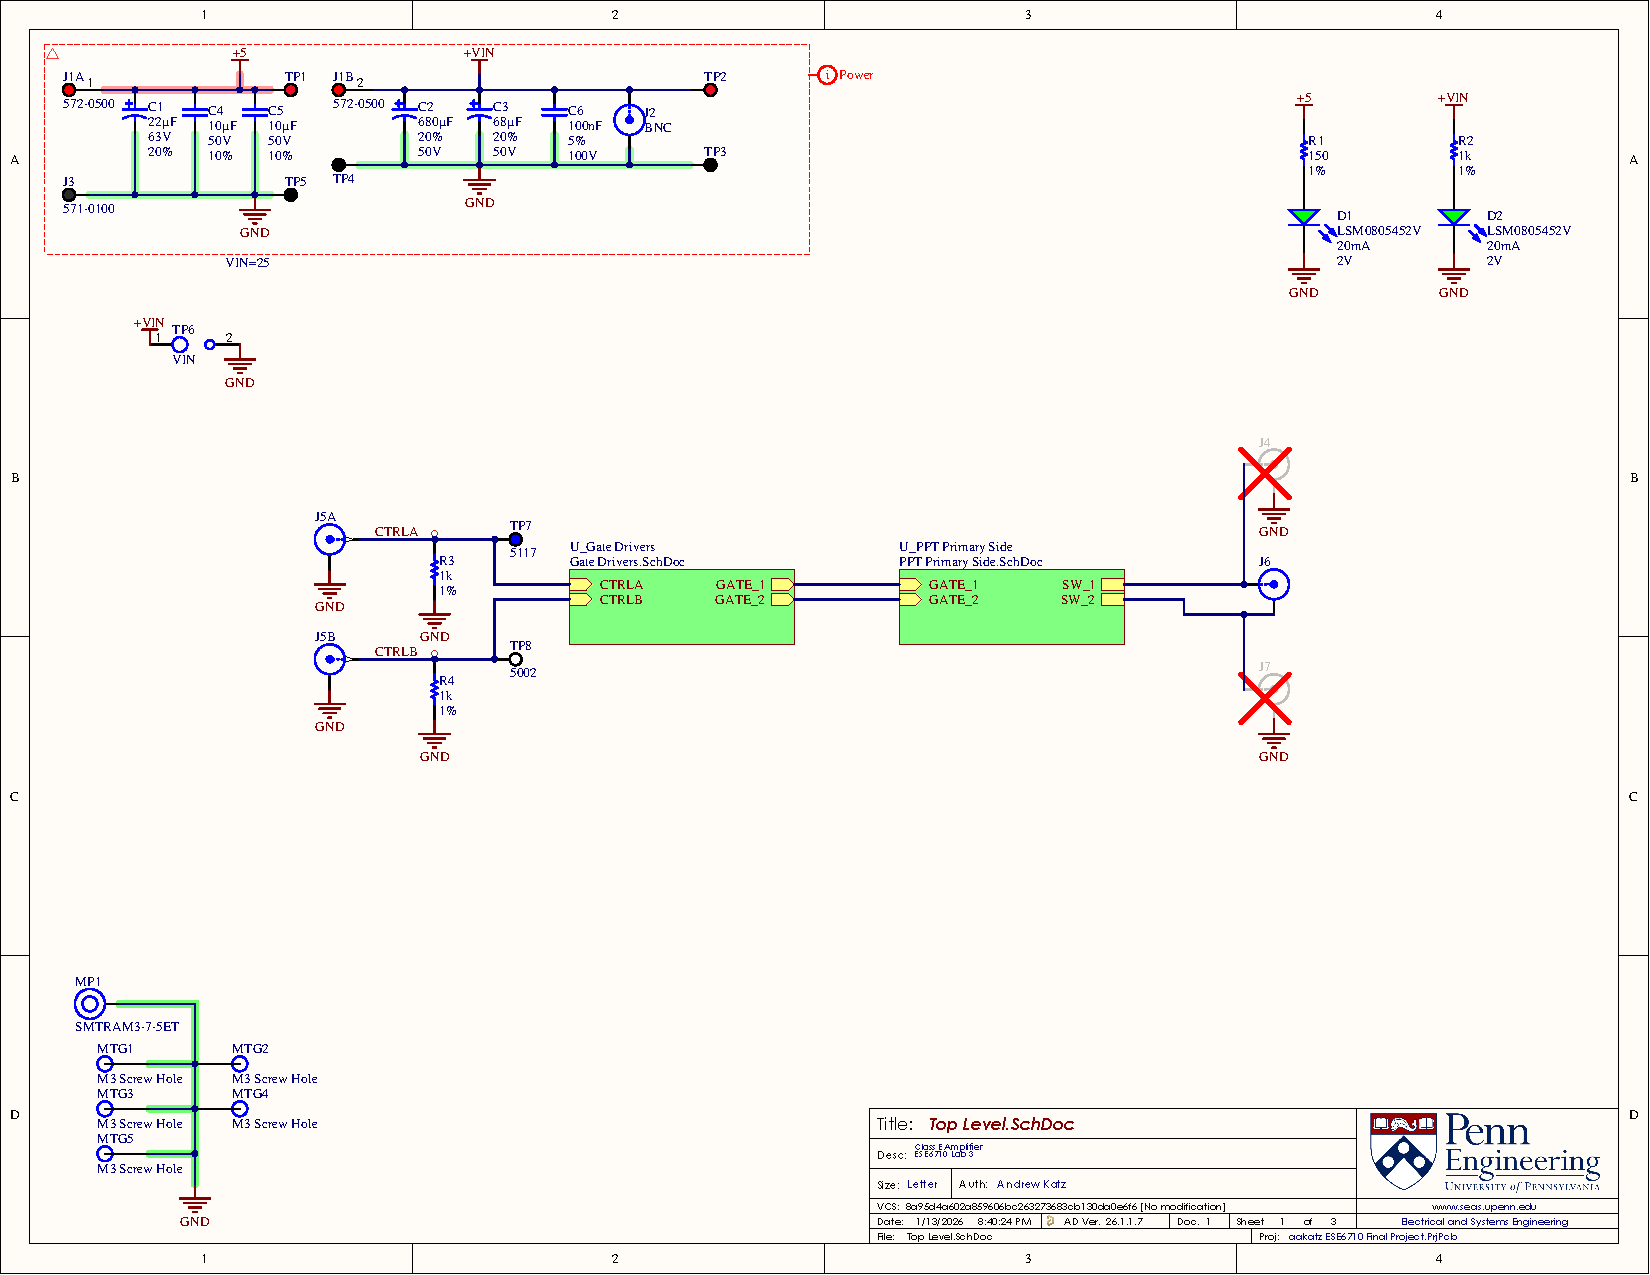
\includegraphics[page=1,width=0.78\linewidth]{figure/sch/inverter_sch.pdf}
        \caption{Top level schematic of the inverter}
    \end{figure}
    \begin{figure}[H]
        \centering
        \includegraphics[page=2,width=0.78\linewidth]{figure/sch/inverter_sch.pdf}
        \caption{Gate Drivers for the inverter}
    \end{figure}
    \begin{figure}[H]
        \centering
        \includegraphics[page=3,width=0.78\linewidth]{figure/sch/inverter_sch.pdf}
        \caption{PPT converter implementation}
    \end{figure}
    \begin{figure}[H]
        \centering
        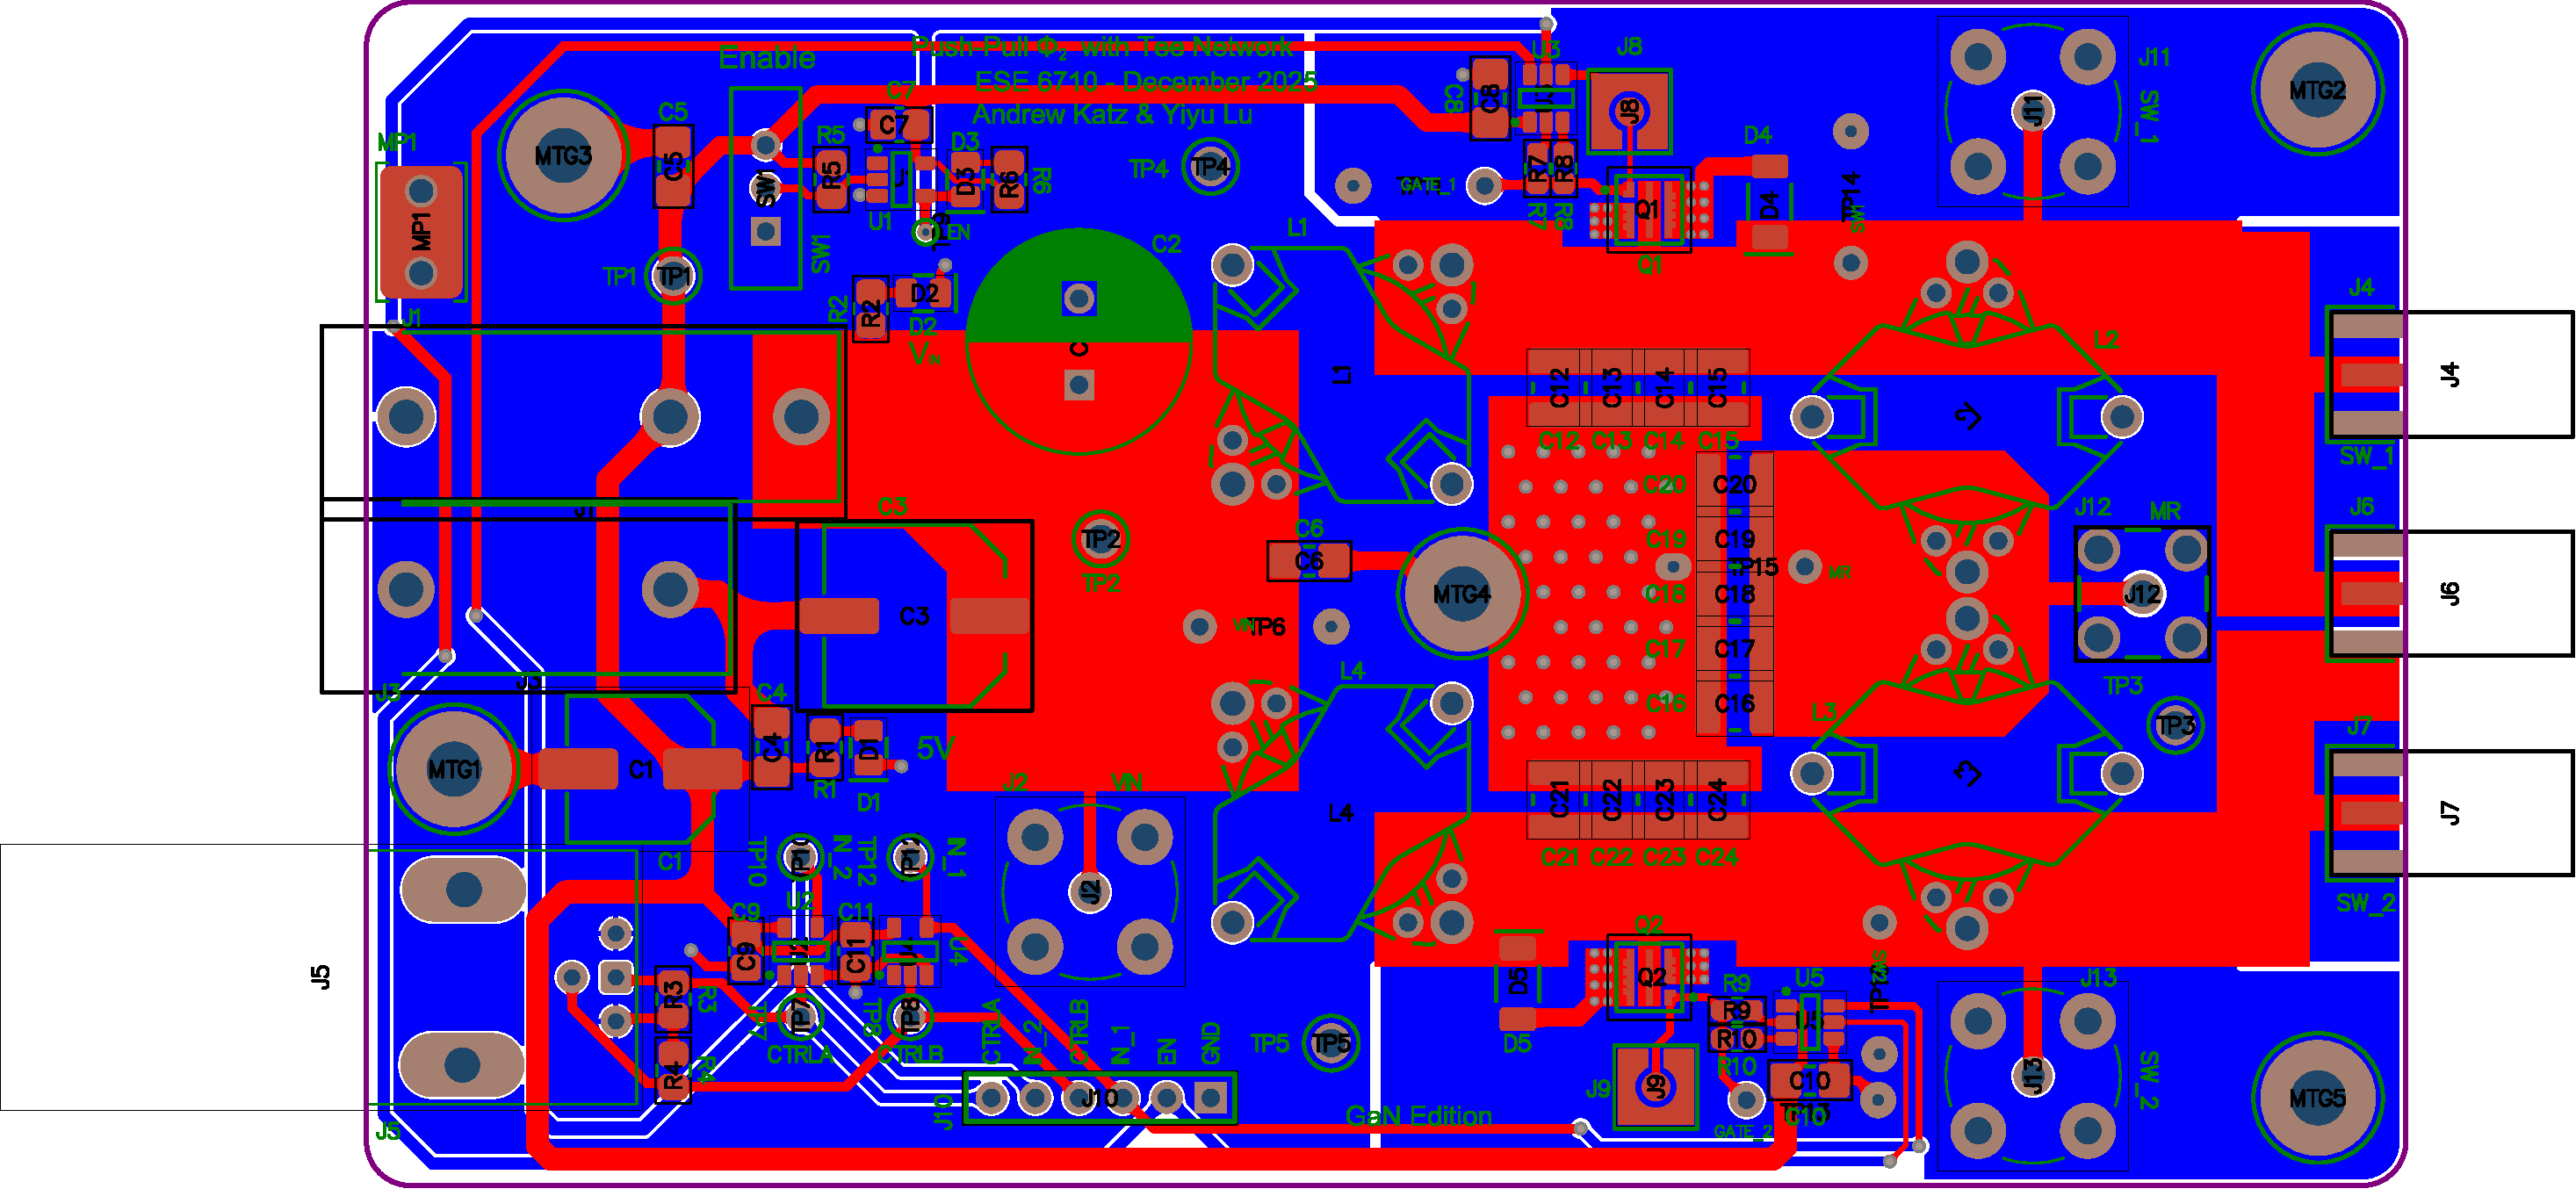
\includegraphics[width=0.8\linewidth]{figure/pcb_layout/inverter-pcb-crop.pdf}
        \caption{PCB Layout of the inverter}
    \end{figure}
    \begin{figure}[H]
        \centering
        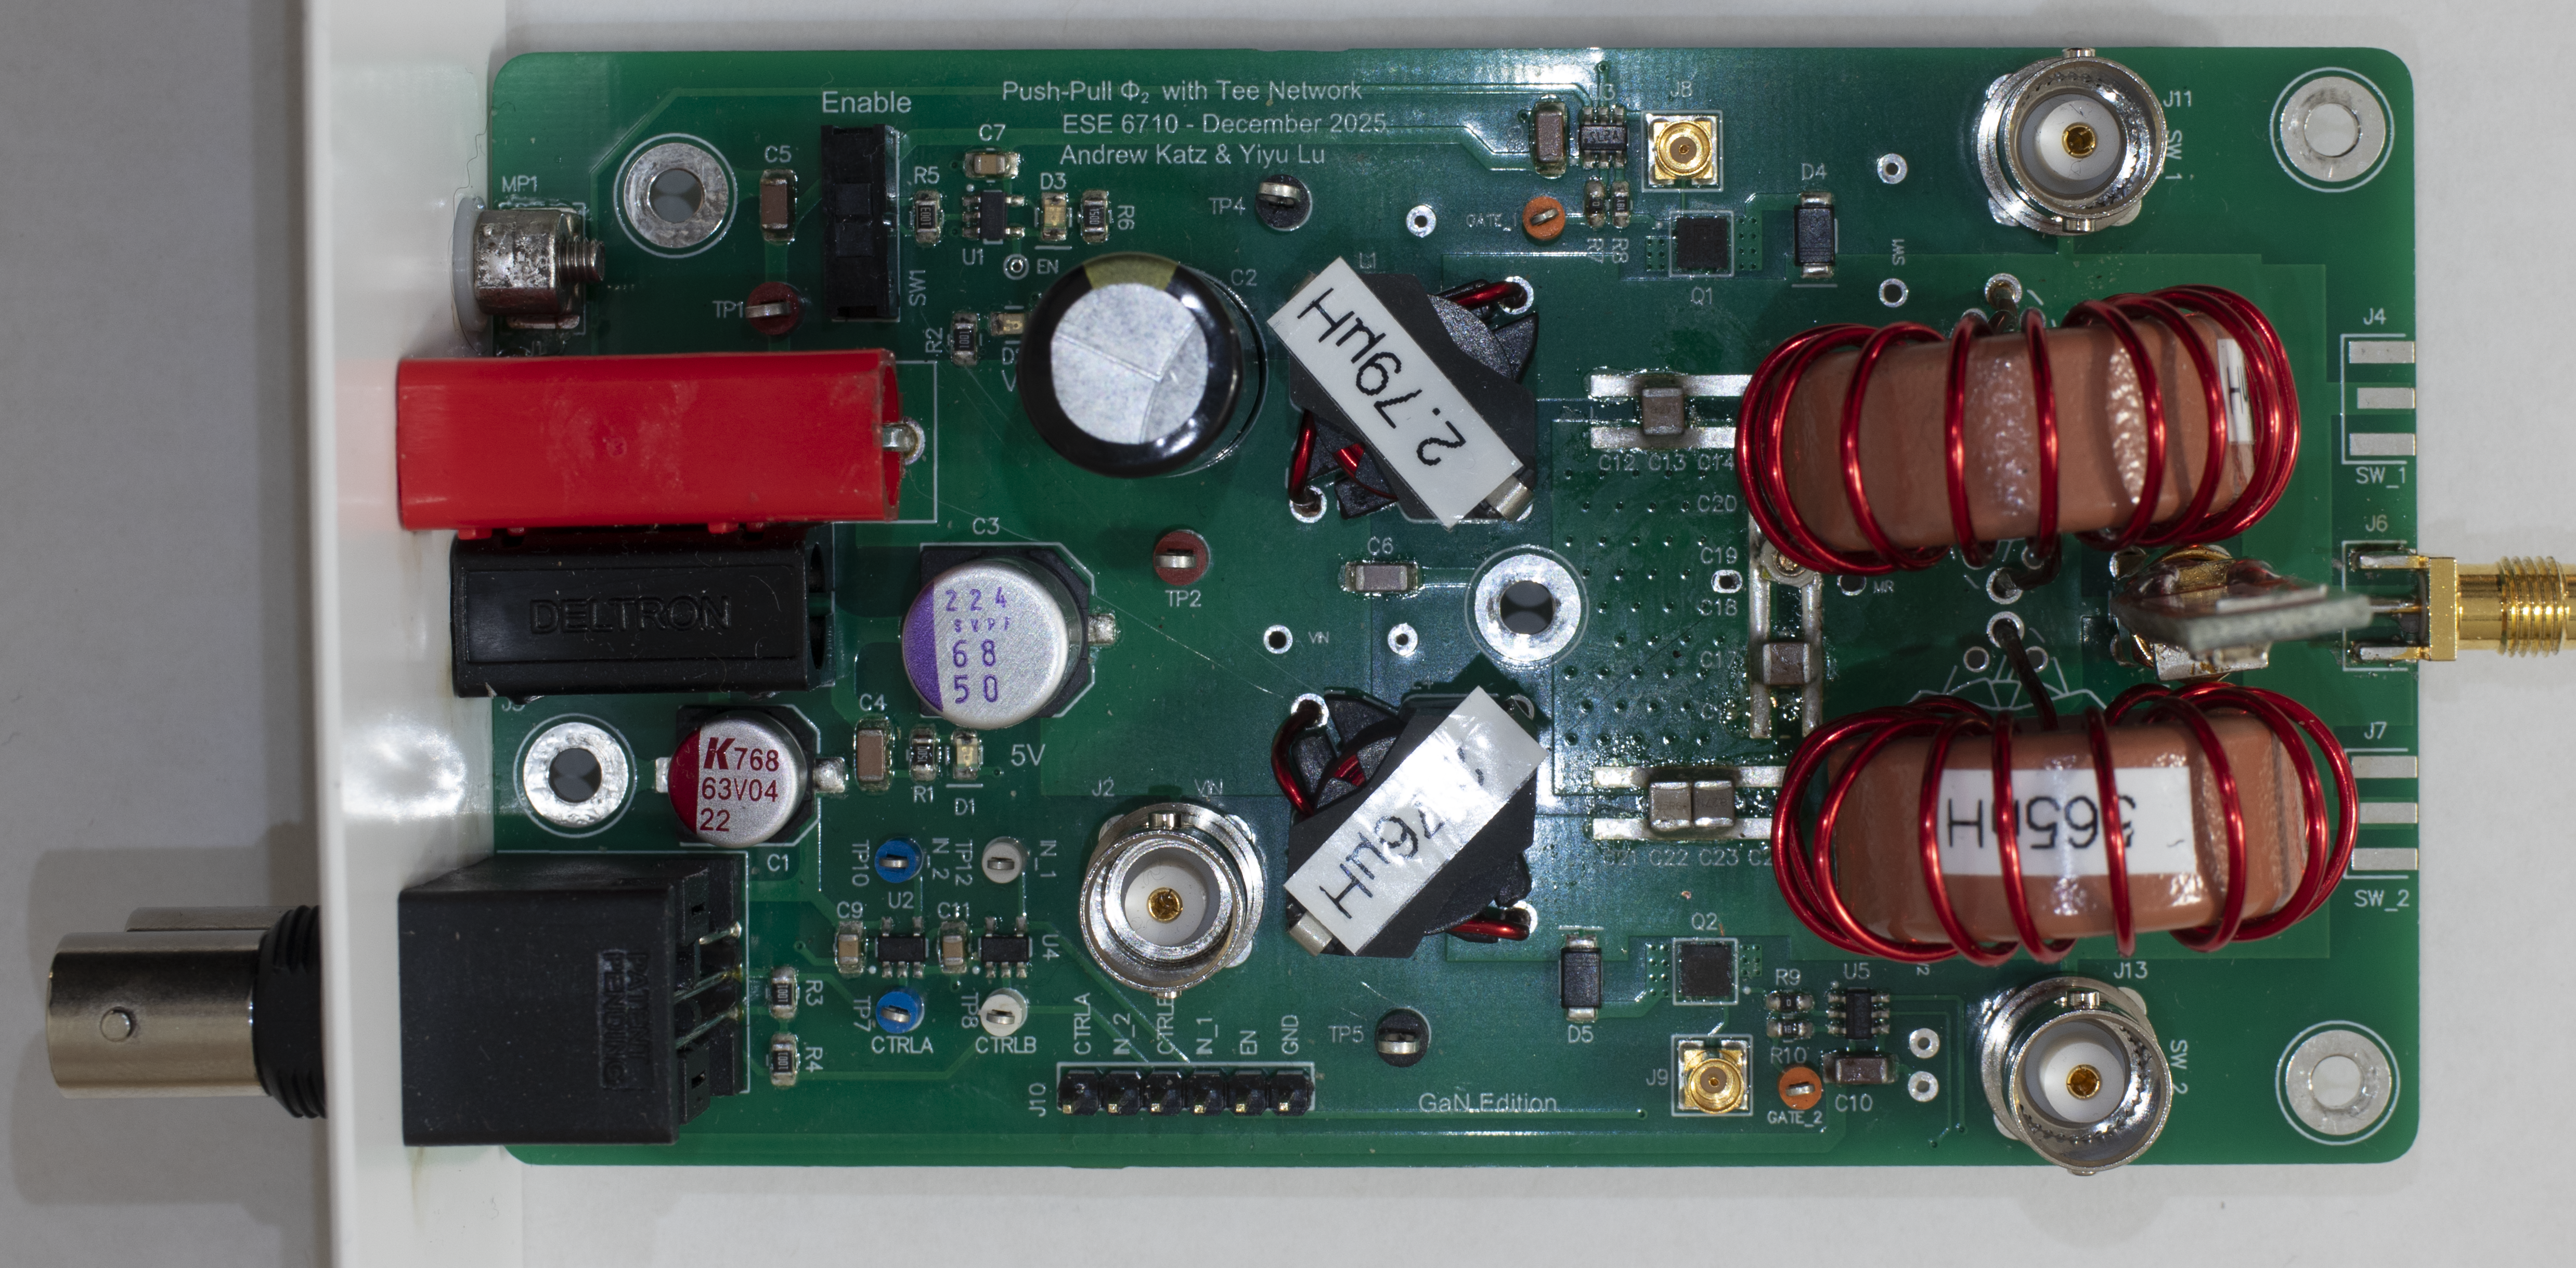
\includegraphics[width=0.8\linewidth]{figure/photo/board/inverter.png}
        \caption{Assembled inverter PCB}
    \end{figure}
    \begin{table}[H]
        \centering
        % !TeX program = luatex
\documentclass{standalone}
\usepackage{booktabs}
\usepackage{longtable}
\usepackage{colortbl}
\usepackage{makecell}
\begin{document}
 
        
            \centering
            \begin{tabular}{lllll}
                \toprule
                 Name & Designator & Value &  Manufacturer & Part Number \\
                 \midrule
                 A768KE226M1JLAE054 & C1 & 22µF &  KEMET & A768KE226M1JLAE054 \\
                 EEU-FC1H681L & C2 & 680µF &  Panasonic & EEUFC1H681L \\
                 50SVPF68M & C3 & 68µF &  Panasonic & 50SVPF68M \\
                 CAP 1206 10UF 50V 10\% X5R & C4, C5 & 10µF &  Samsung Electro-Mechanics & CL31A106KBHNNNE \\
                 CAP 1206 0.1UF 100V 5\% C0G & C6 & 100nF &  TDK & C3216C0G2A104J160AC \\
                 CAP 0805 0.1UF 50V 10\% X7R & C7, C9, C11 & 100nF &  Yageo Group & CC0805KRX7R9BB104 \\
                 CAP 1206 1.0UF 50V 10\% X7R & C8, C10 & 1µF &  Samsung Electro-Mechanics & CL31B105KBHNNNE \\
                 800B271JT200XT & C13, C22 & 270pF &  KYOCERA AVX & 800B271JT200XT \\
                 800B471JT200XT1K & C17 & 470pF &  KYOCERA AVX & 800B471JT200XT1K \\
                 JR500HV & C18 & 8pF-50pF &  Voltronics & JR500HV \\
                 800B5R6CT500XT & C23 & 5.6pF &  KYOCERA AVX & 800B5R6CT500XT \\
                 LSM0805452V & D1, D2, D3 &  &  VCC & LSM0805452V \\
                 RB058LAM100TFTR & D4, D5 &  &  ROHM & RB058LAM100TFTR \\
                 572-0500 & J1 &  &  Deltron & 572-0500 \\
                 BNC THT Vertical & J2, J11, J13 & 50Ω &  Amphenol RF & B6251C1-NT3G-50 \\
                 571-0100 & J3 &  &  Deltron & 571-0100 \\
                 031-6575 & J5 &  &  Amphenol RF & 031-6575 \\
                 CON-SMA-EDGE-S & J6 &  &  RF Solutions & CON-SMA-EDGE-S \\
                 135-3711-201 & J8, J9 &  &  Cinch Connectivity Solutions & 135-3711-201 \\
                 MHDR 1X6 & J10 &  &  Adam Tech & PH1-06-UA \\
                 RF2-04A-T-00-50-G & J12 &  &  Adam Tech & RF2-04A-T-00-50-G \\
                 RM6 Custom Inductor, K1 Core & L1, L4 & 2.754µH, 2.7857µH &  \makecell{TDK EPCOS\\ TDK EPCOS\\ Remington Industries} & \makecell{B65808N1006D001 \\ B65807N0040A001 \\ 18HNS} \\
                 Toroidal Custom Inductor, T106-0 Core & L2, L3 & 564.97nH, 566.72nH &  \makecell{Micrometals \\ Remington Industries} & \makecell{T106-0 \\ 18HNS} \\
                 SMTRAM3-7-5ET & MP1 &  &  PEM PennEngineering & SMTRAM3-7-5ET \\
                 IGB110S101XTMA1 & Q1, Q2 &  &  Infineon & IGB110S101XTMA1 \\
                 RES 0805 150 1\% & R1, R6 & 150Ω &  Stackpole Electronics & RMCF0805FT150R \\
                 RES 0805 1K 1\% & R2, R3, R4 & 1kΩ &  Stackpole Electronics & RMCF0805FT1K00 \\
                 RES 0805 100K 1\% & R5 & 100kΩ &  TE Connectivity & CRG0805F100K \\
                 RES 0603 0 & R7, R9 & 0Ω &  Stackpole Electronics & RMCF0603ZT0R00 \\
                 RES 0603 1.5 1\% & R8, R10 & 1.5Ω &  Stackpole Electronics & RMCF0603FT1R50 \\
                 EG1218 & SW1 &  &  E-Switch & EG1218 \\
                 5280 & TP1, TP2 &  &  Keystone & 5280 \\
                 5281 & TP3, TP4, TP5 &  &  Keystone & 5281 \\
                 5117 & TP7, TP10 &  &  Keystone & 5117 \\
                 5002 & TP8, TP12 &  &  Keystone & 5002 \\
                 SN74LVC1G04DBVR & U1 &  &  Texas Instruments & SN74LVC1G04DBVR \\
                 SN74LVC1G34DBVR & U2, U4 &  &  Texas Instruments & SN74LVC1G34DBVR \\
                 LM5114AMF/NOPB & U3, U5 &  &  Texas Instruments & LM5114AMF/NOPB \\
                 \bottomrule                
            \end{tabular}
        
        

\end{document}
        \caption{BOM of the inverter}
    \end{table}
    %    \FloatBarrier
    \subsection{Coil Interface}
    \begin{figure}[H]
        \centering
        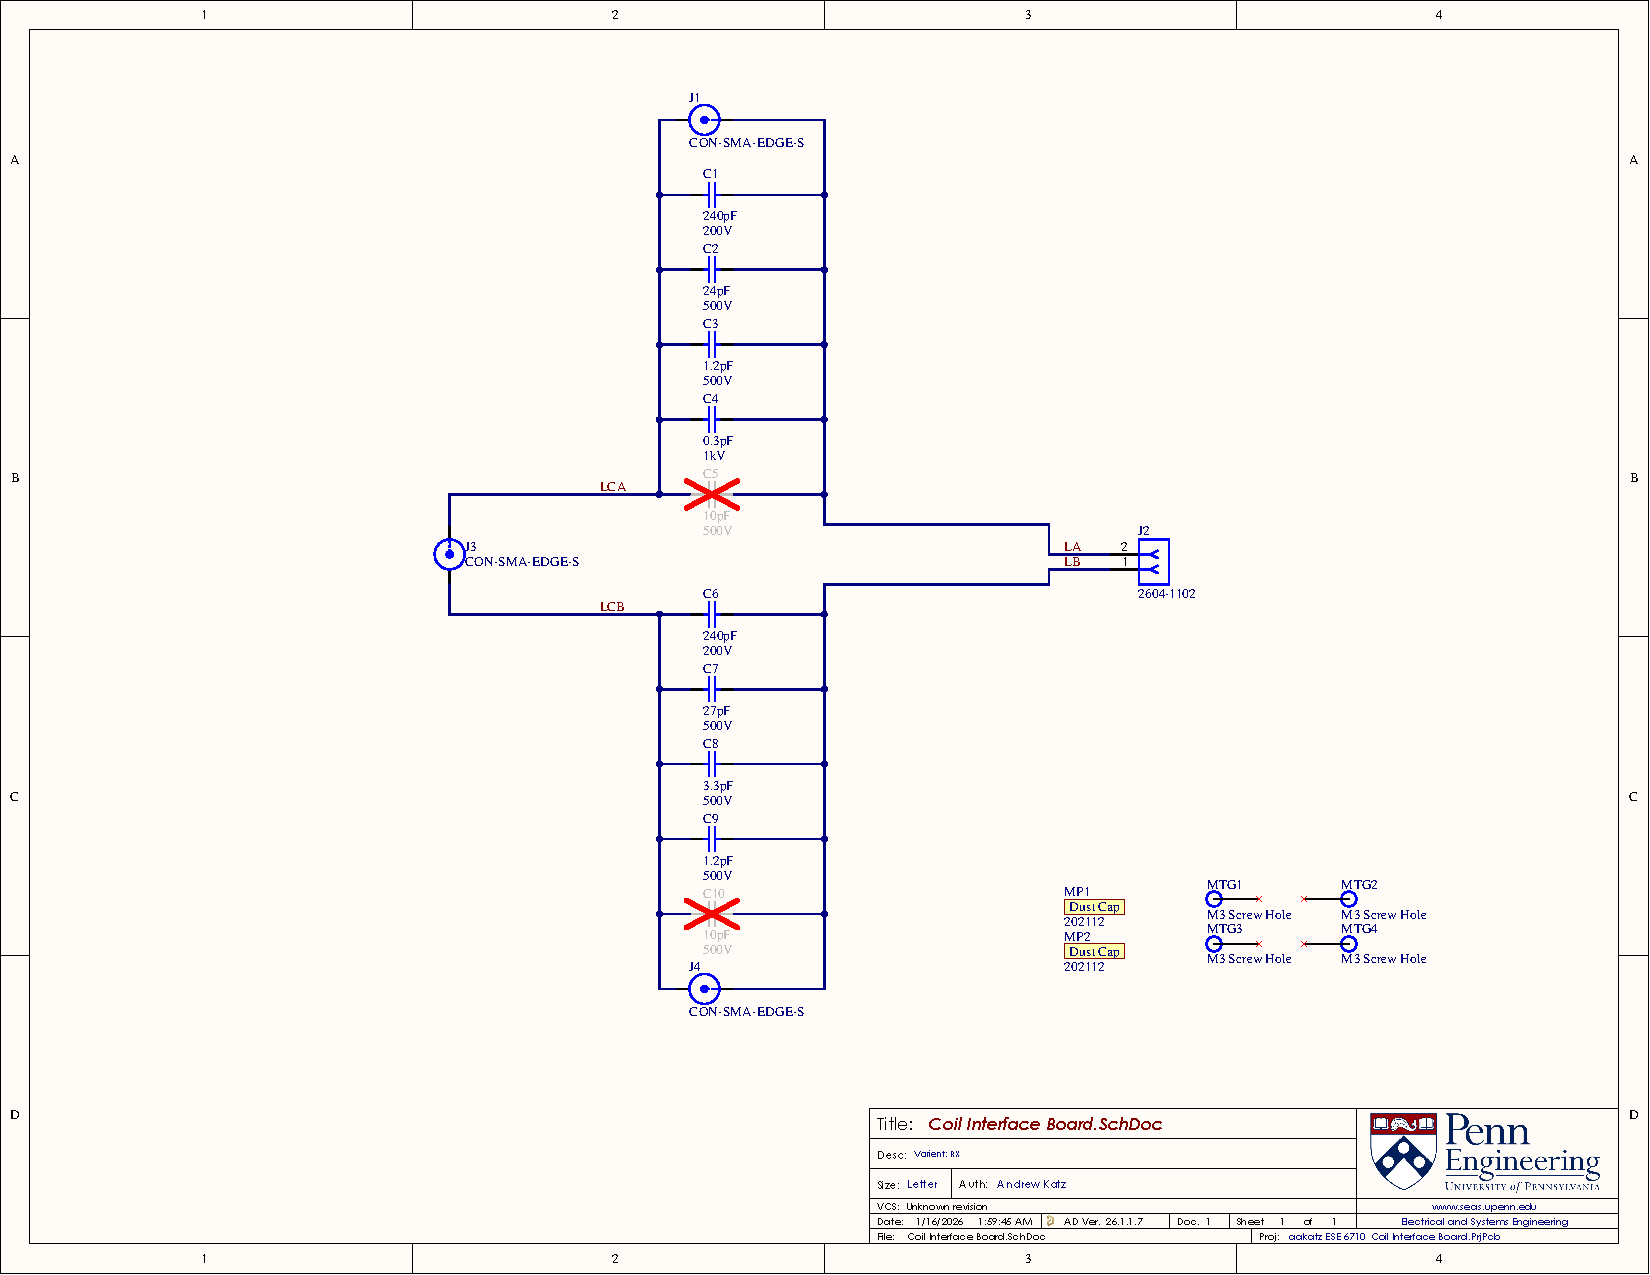
\includegraphics[page=1,width=0.78\linewidth]{figure/sch/Coil-Interface-SCH.pdf}
        \caption{Schematic of the coil interface, receiver side (RX)}
    \end{figure}
    \begin{figure}[H]
        \centering
        \includegraphics[page=2,width=0.78\linewidth]{figure/sch/Coil-Interface-SCH.pdf}
        \caption{Schematic of the coil interface, transmitter side (TX)}
    \end{figure}
    \begin{figure}[H]
        \centering
        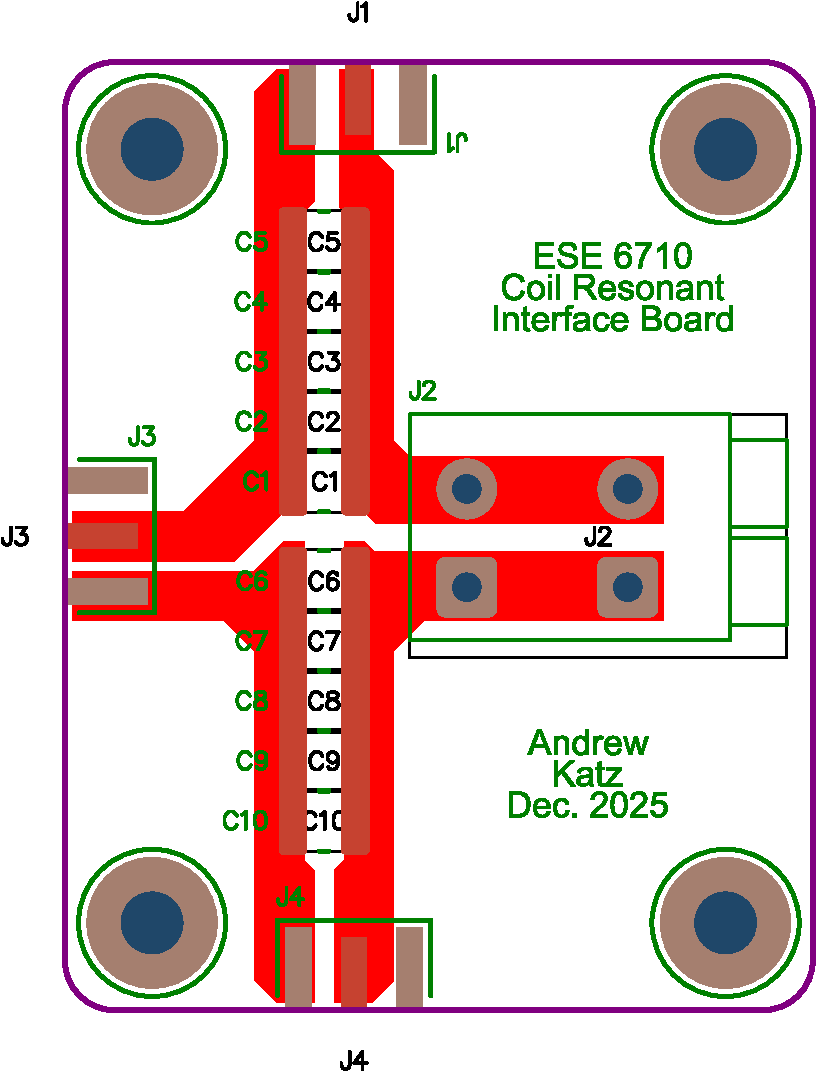
\includegraphics[width=0.3\linewidth]{figure/pcb_layout/Coil-Interface-PCB.pdf}
        \caption{PCB Layout of the coil interface}
    \end{figure}
    \begin{figure}[H]
        \centering
        \subfloat[]{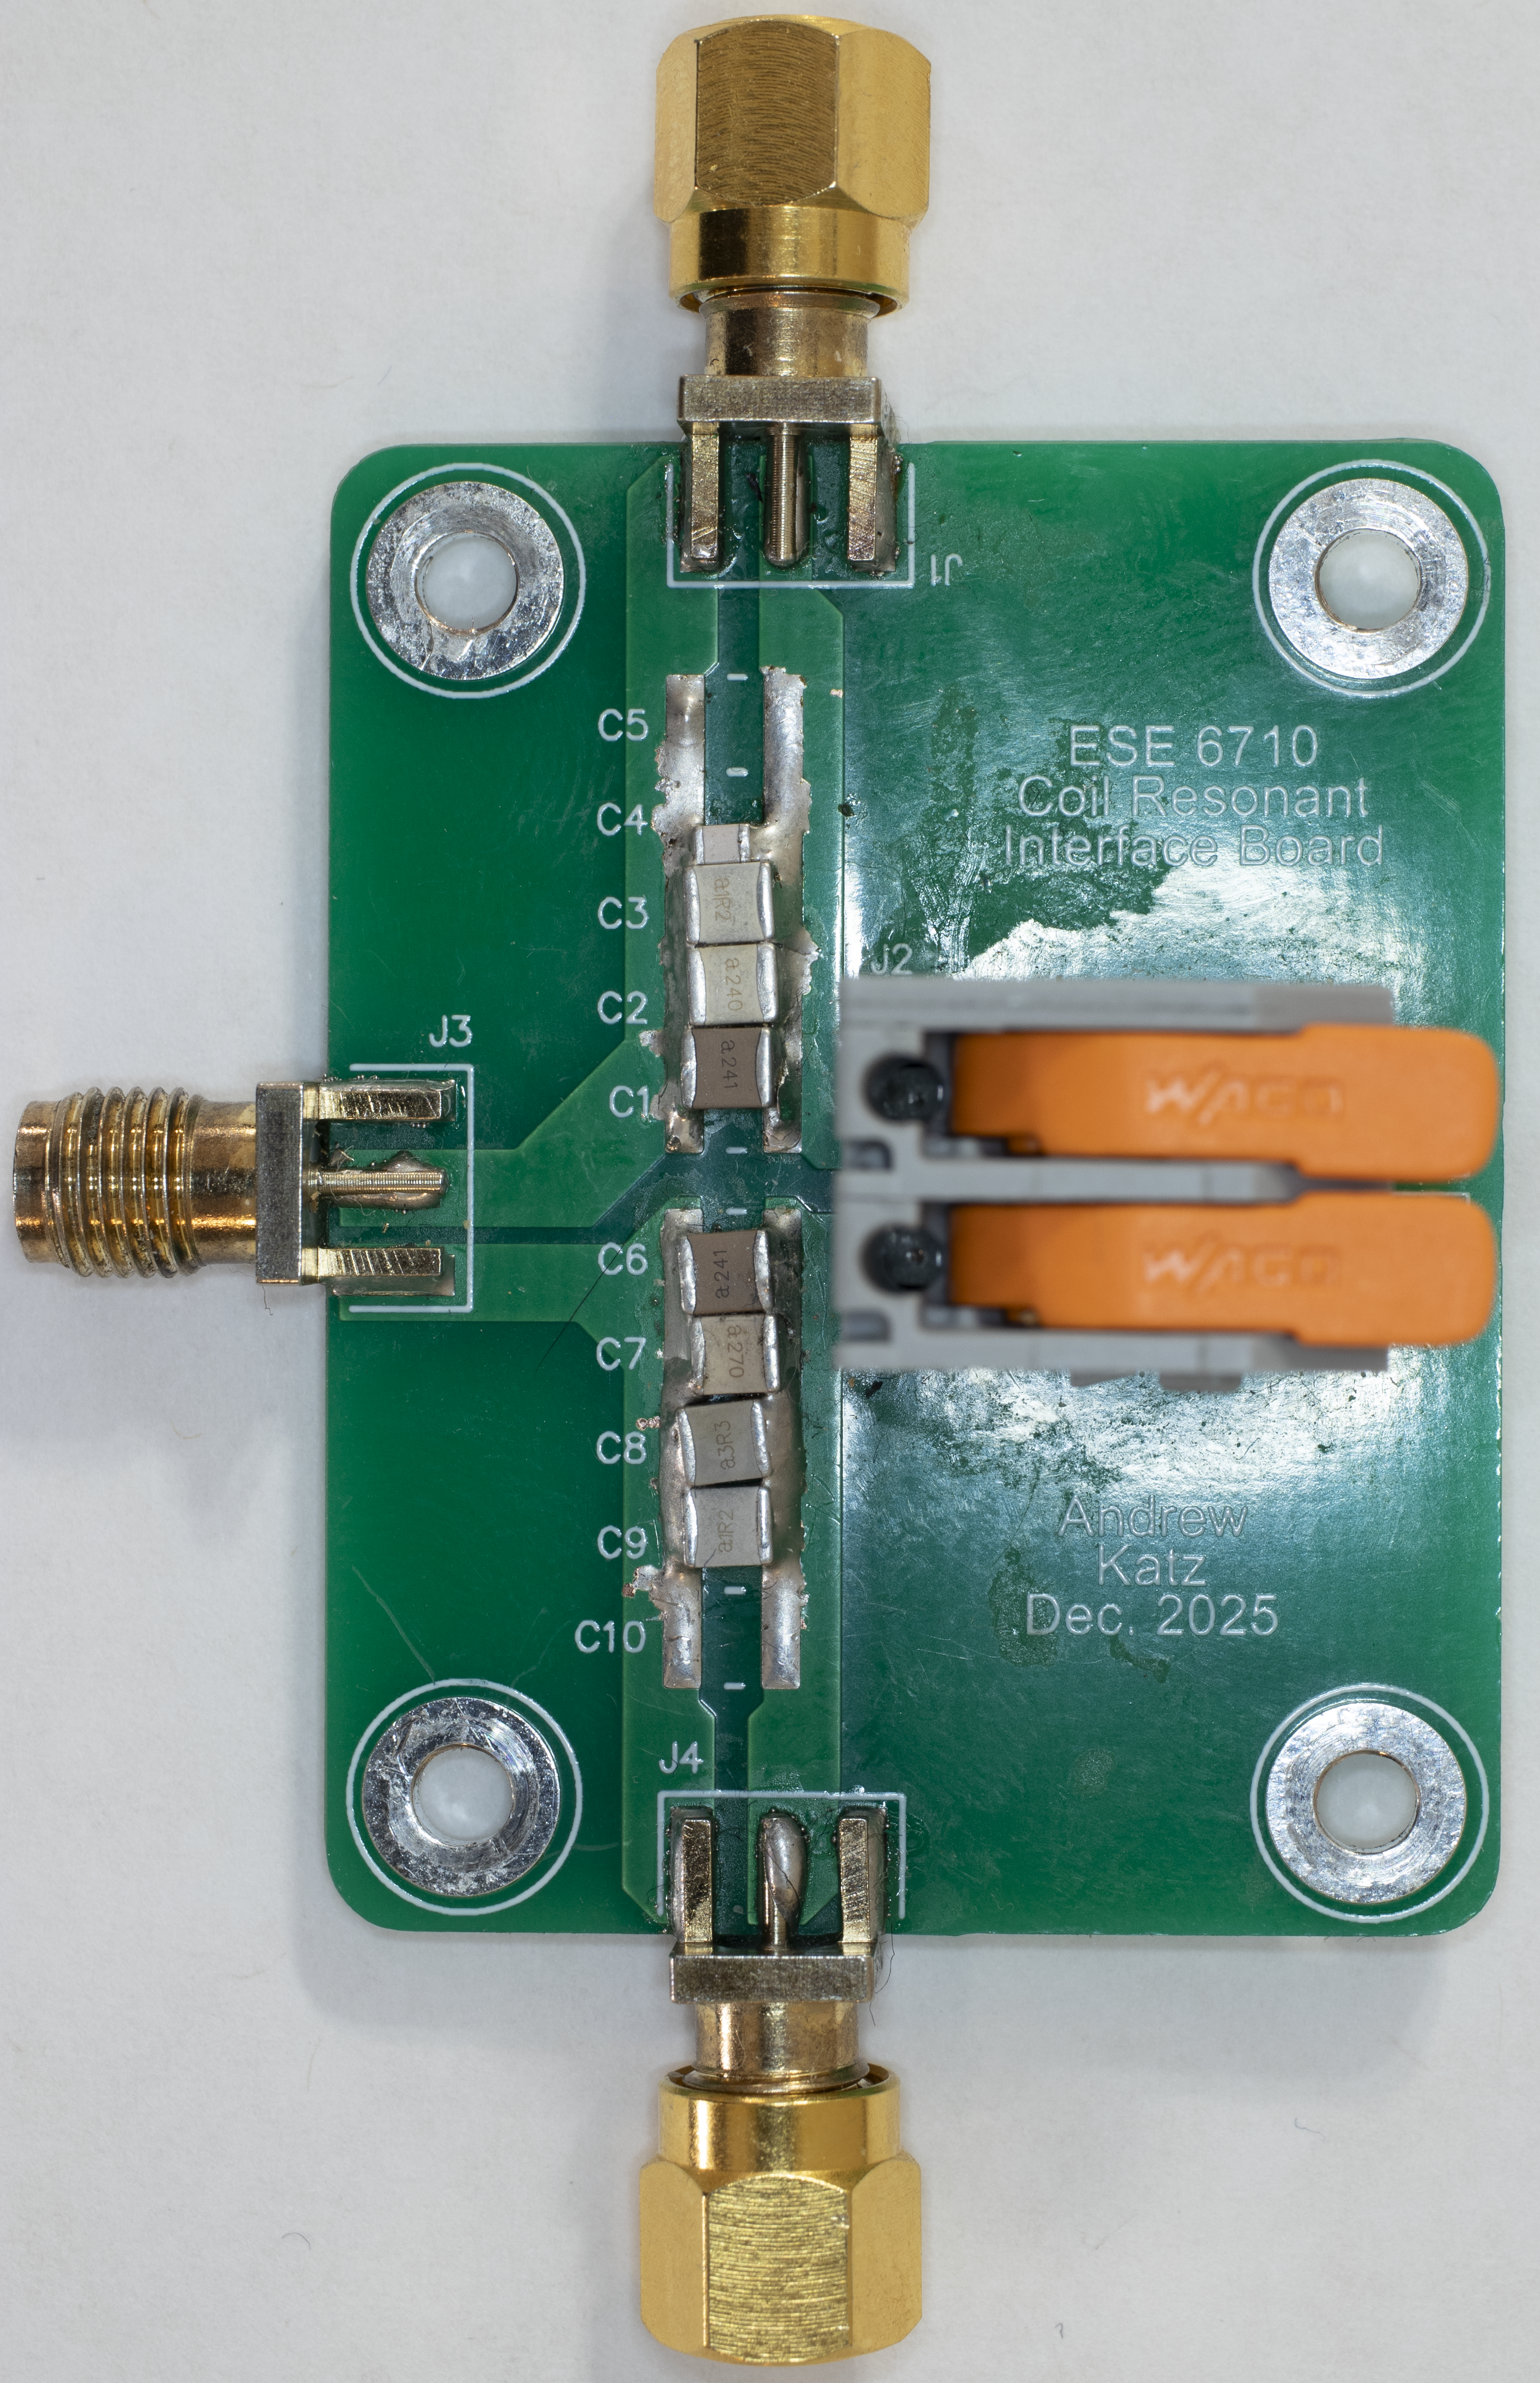
\includegraphics[height=144pt]{figure/photo/board/RX.png}\label{fig:board:RX}}
        \hfil
        \subfloat[]{\includegraphics[height=144pt]{figure/photo/board/TX.png}\label{fig:board:TX}}
        \caption{
            \centering
            Assembled coil interface:\quad
            (a)\; RX\quad
            (b)\; TX
        }
    \end{figure}
    \begin{table}[H]
        \centering
        % !TeX program = luatex
\documentclass{standalone}
\usepackage{booktabs}
\usepackage{longtable}
\usepackage{colortbl}
\usepackage{makecell}
\begin{document}
    \centering
    
\end{document}
        \caption{BOM for TX and RX configurations of the coil interface}
    \end{table}
    %    \FloatBarrier
    
    \subsection{Rectifier}
    
    \begin{figure}[H]
        \centering
        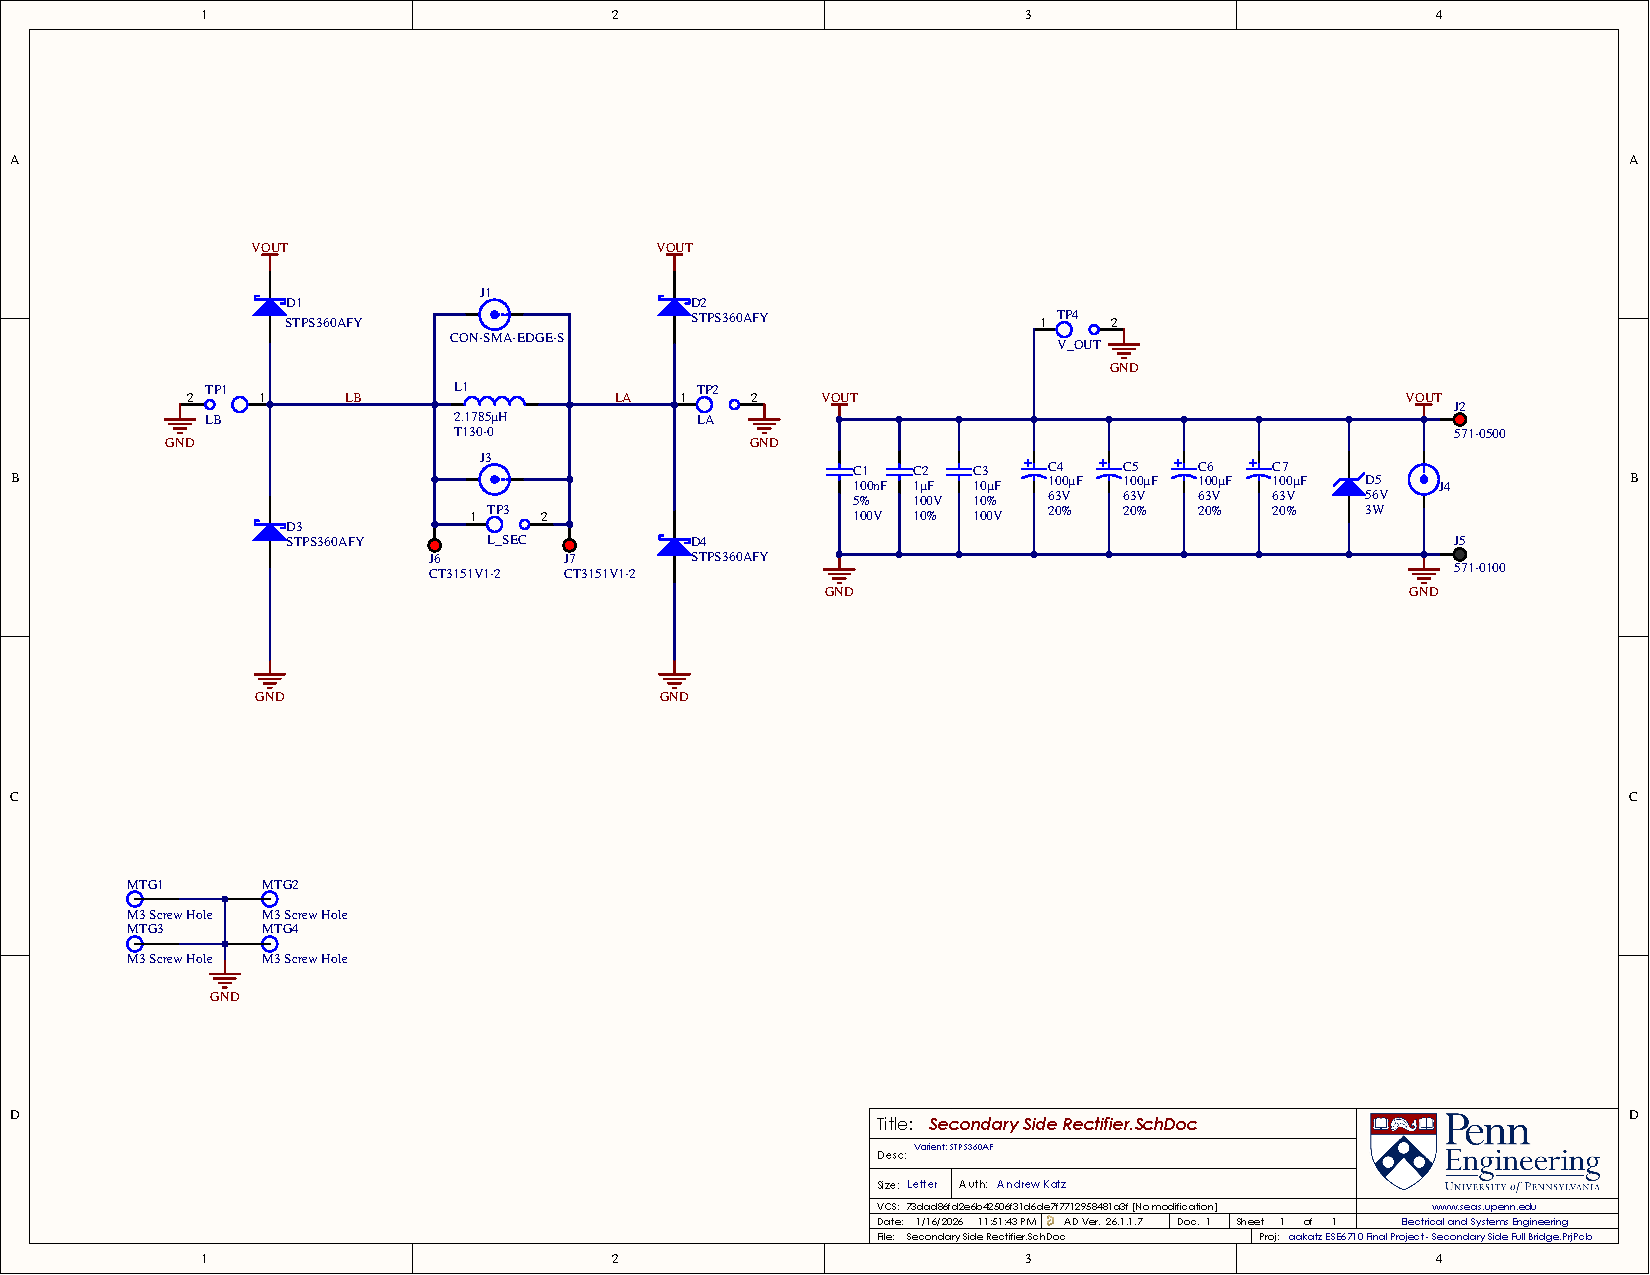
\includegraphics[page=1,width=0.78\linewidth]{figure/sch/Rectifier-SCH.pdf}
        \caption{Rectifier, STPS360AF variant (used)}
    \end{figure}
    \begin{figure}[H]
        \centering
        \includegraphics[page=2,width=0.78\linewidth]{figure/sch/Rectifier-SCH.pdf}
        \caption{Rectifier, RB058LAM100TFTR variant (not used)}
    \end{figure}
    \begin{figure}[H]
        \centering
        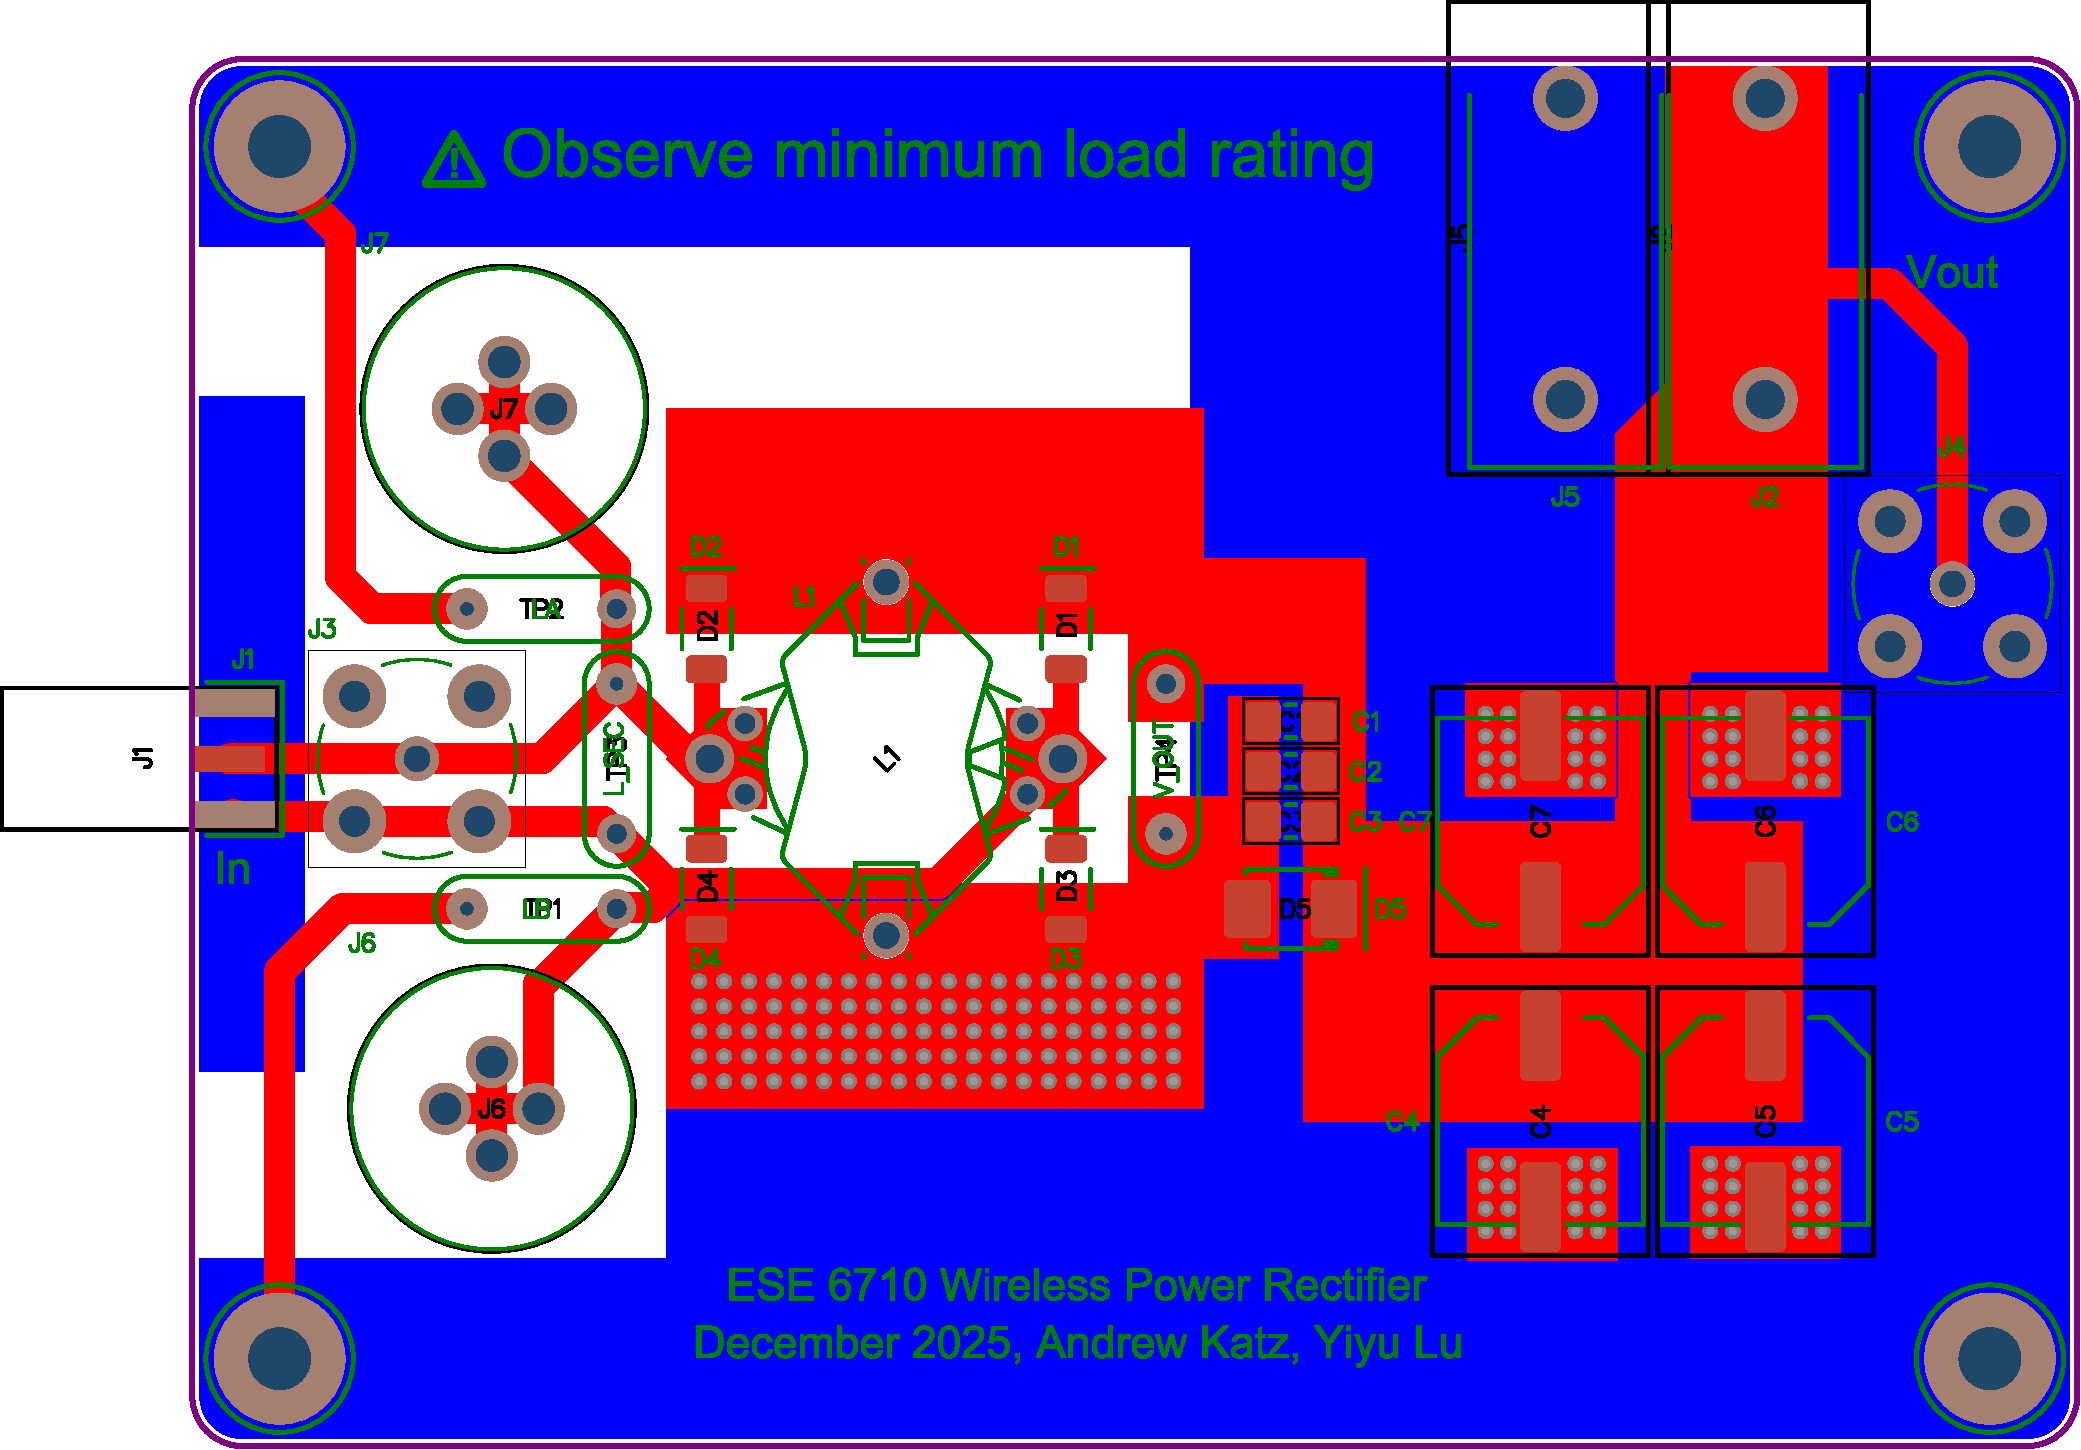
\includegraphics[width=0.5\linewidth]{figure/pcb_layout/Rectifier-PCB.pdf}
        \caption{PCB Layout of the rectifier}
    \end{figure}
    \begin{figure}[H]
        \centering
        \subfloat[]{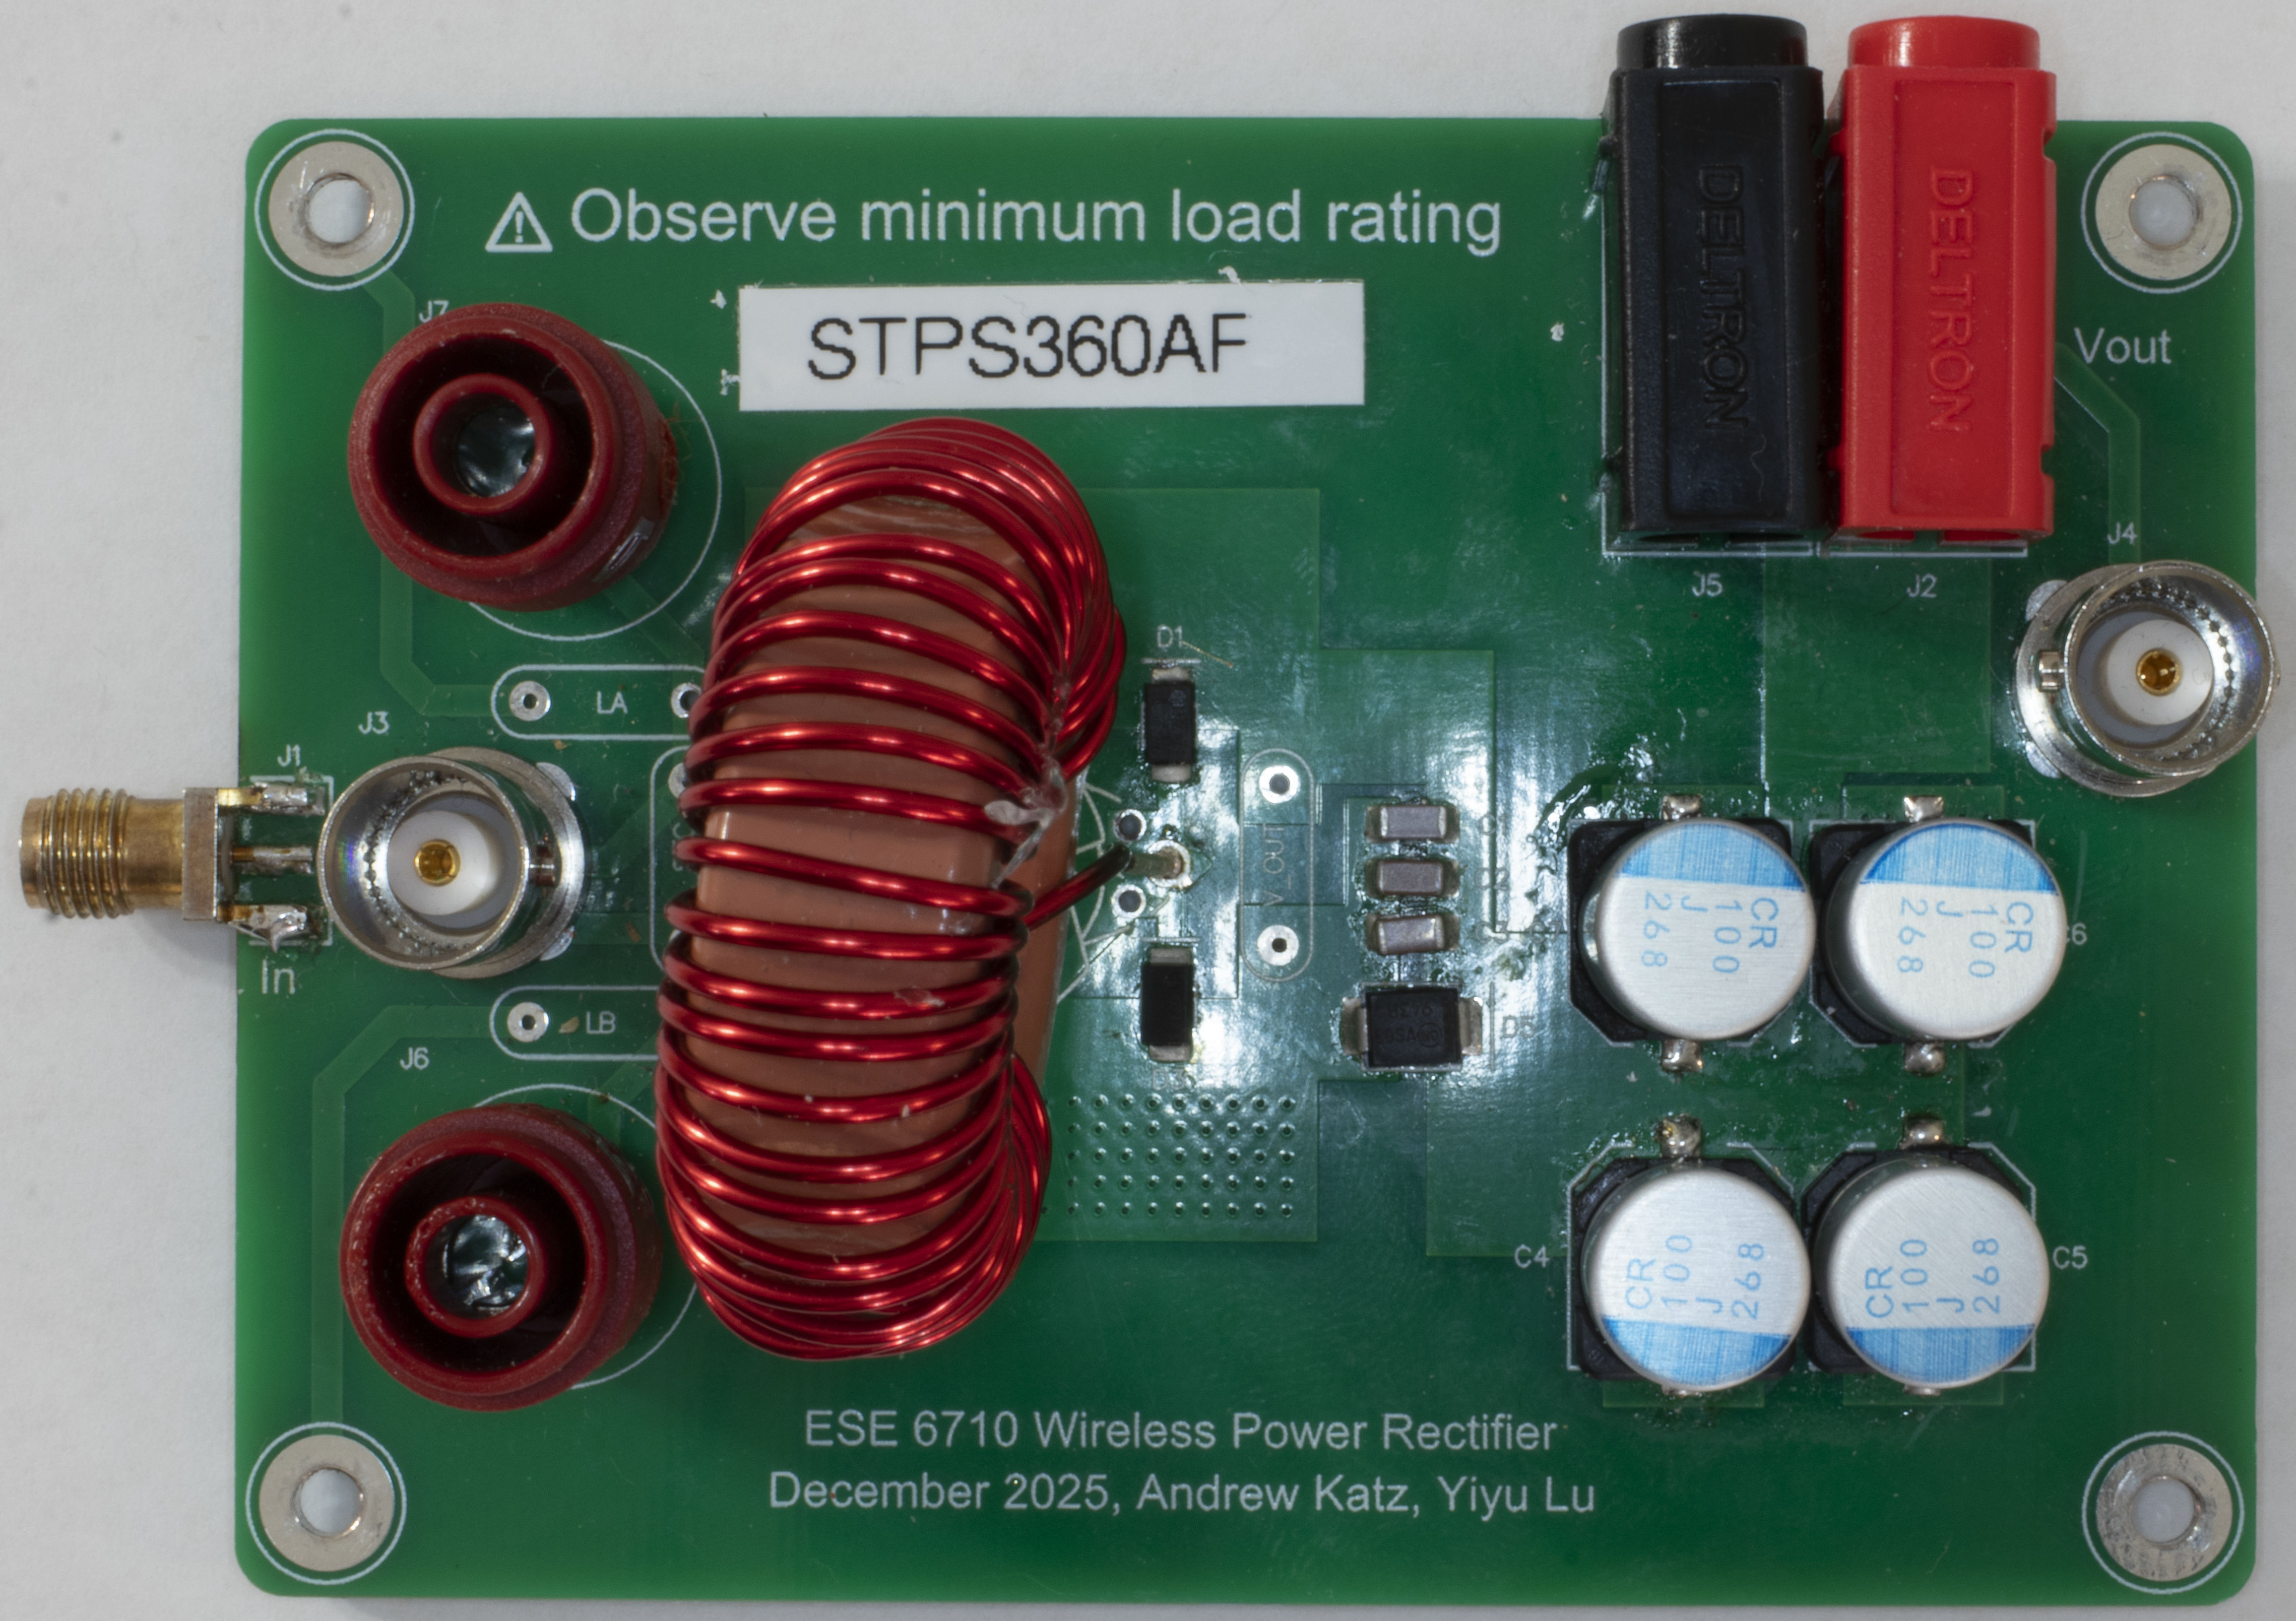
\includegraphics[height=144pt]{figure/photo/board/rectifier.png}}
        \hfil
        \subfloat[]{\includegraphics[height=144pt]{figure/photo/board/rectifier2.png}}
        \caption{
            \centering
            Assembled rectifier:\quad
            (a)\; Rectifier, STPS360AF variant (used)\quad
            (b)\; Rectifier, RB058LAM100TFTR variant (not used in final configuration)
        }
    \end{figure}
    \begin{table}[H]
        \centering
        % !TeX program = luatex
\documentclass{standalone}
\usepackage{booktabs}
\usepackage{longtable}
\usepackage{colortbl}
\usepackage{makecell}
\begin{document}
\centering

\begin{tabular}{lccccl}
	\toprule
	\textbf{Name}                & \textbf{Designator} & \textbf{Varient} & \textbf{Value} & \textbf{Manufacturer} & \textbf{Part Number} \\
	\midrule
	CAP 1206 0.1UF 100V 5\% C0G  & C1                  & All              & 100nF          & TDK                   & C3216C0G2A104J160AC  \\
	CAP 1206 1.0UF 100V 10\% X7R & C2                  & All              & 1µF            & TDK                   & C3216X7R2A105K160AA  \\
	CAP 1206 10UF 100V 10\% X6S  & C3                  & All              & 10µF           & TDK                   & C3216X6S2A106K160AC  \\
	PCR1J101MCL1GS               & C4, C5, C6, C7      & All              & 100µF          & Nichicon              & PCR1J101MCL1GS       \\
	RB058LAM100TFTR              & D1, D2, D3, D4      & RB058LAM100TFTR  &                & ROHM                  & RB058LAM100TFTR      \\
	STPS360AFY                   & D1, D2, D3, D4      & STPS360AF        &                & STMicroelectronics    & STPS360AFY           \\
	1SMB5946BT3G                 & D5                  & RB058LAM100TFTR  &                & onsemi                & 1SMB5946BT3G         \\
	1SMB5943BT3G                 & D5                  & STPS360AF        &                & onsemi                & 1SMB5943BT3G         \\
	CON-SMA-EDGE-S               & J1                  & All              &                & RF Solutions          & CON-SMA-EDGE-S       \\
	571-0500                     & J2                  & All              &                & Deltron               & 5710500              \\
	BNC THT Vertical             & J3, J4              & All              & 50O            & Amphenol RF           & B6251C1-NT3G-50      \\
	571-0100                     & J5                  & All              &                & Deltron               & 571-0100             \\
	CT3151V1-2                   & J6, J7              & All              &                & Cal Test Electronics  & CT3151V1-2           \\
	Custom Inductor, T130-0 Core & L1                  & All              & 2.1785µH       & Micrometals           & T130-0               \\
	\bottomrule
\end{tabular}
\end{document}
        \caption{BOM for the rectifier}
    \end{table}
    %    \FloatBarrier
    \newpage
    \subsection{Probe Capacitance Emulator}
    
    \begin{figure}[H]
        \centering
        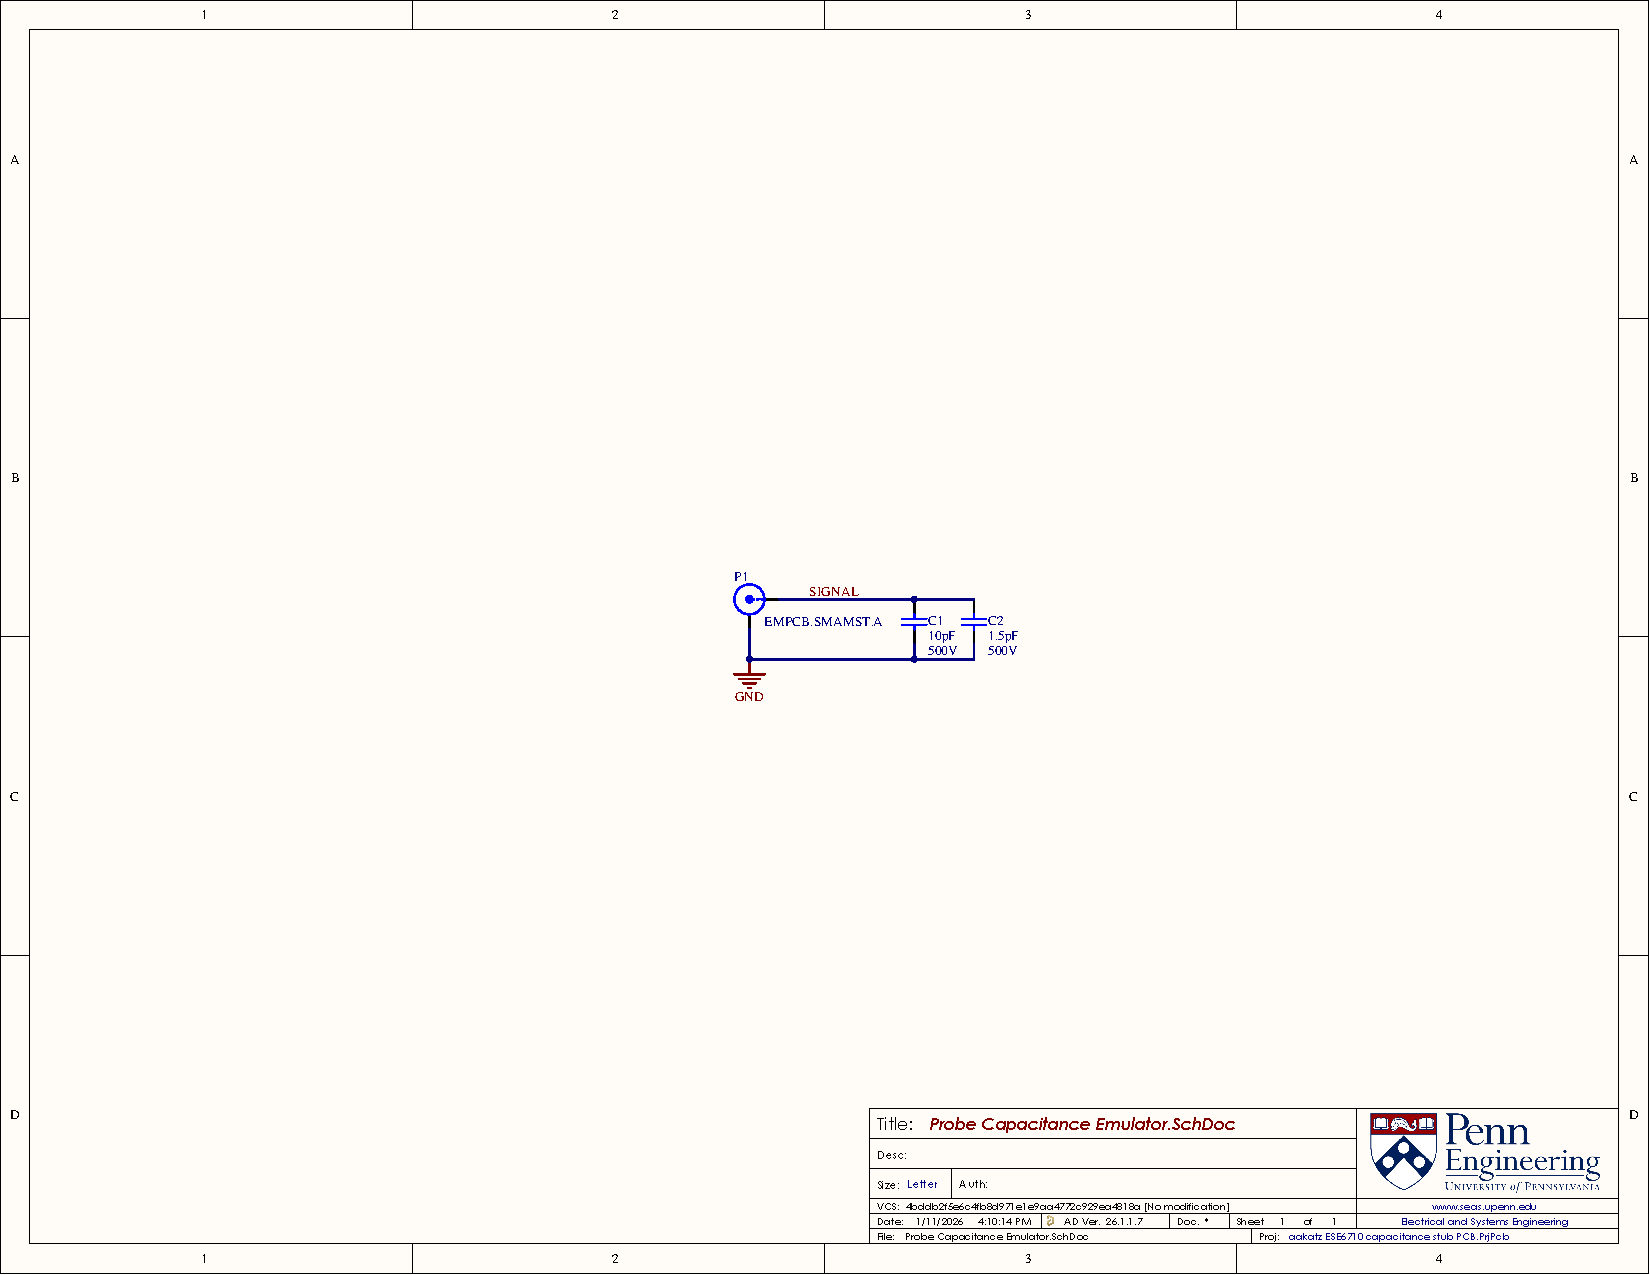
\includegraphics[trim=4.5in 3.75in 4in 3.5in, clip, width=0.5\linewidth]{figure/sch/capacitance-emulator-sch.pdf}
        \caption{Schematic of probe capacitance emulator to emulate the effect of a \texttt{Keysight 10073D} passive probe, \texttt{Cal Test Electronics CT2708}, and a \texttt{Mini-Circuits SM-BF50+}}
        \label{fig:sch:probe-capacitance-emulator}
    \end{figure}
    
    \begin{figure}[H]
        \centering
        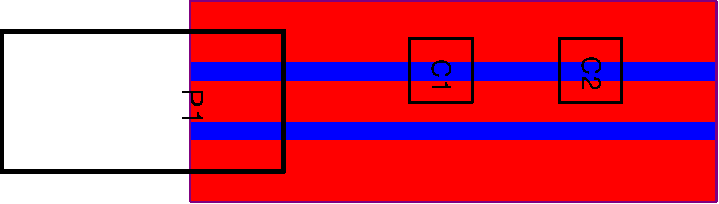
\includegraphics[width=0.4\linewidth]{figure/pcb_layout/capacitance-emulator-pcb.pdf}
        \caption{CAD drawing of PCB layout for the probe capacitance emulator}
        \label{fig:pcb:probe-capacitance-emulator}
    \end{figure}
    
    \begin{figure}[H]
        \centering
        \subfloat[]{\includegraphics[width=0.4\linewidth]{figure/photo/board/IMG_0010_edit.PNG}\label{fig:board:probe-capacitance-emulator:front}}
        \hfil
        \subfloat[]{\includegraphics[width=0.4\linewidth]{figure/photo/board/IMG_0012_edit.PNG}\label{fig:board:probe-capacitance-emulator:rear}}
        
        \caption{
            \centering
            Assembled probe capacitance emulator:\quad
            (a) Front
            (b) Back
        }
        \label{fig:cap-em}
    \end{figure}
    
    \begin{table}[H]
        \centering
        \csvreader[head to column names,tabular=cccc, table head=\toprule\bfseries Component Designator & \bfseries Value & \bfseries Manufacturer & \bfseries Part Number\\ \midrule,table foot=\bottomrule,]
        {table/bom/BOM-ProbeEmulator.csv}{}%
        {\Designator & \Value & \Manufacturer & \ManufacturerPartNumber}
        \caption{Bill of Materials for the probe capacitance emulator}
        \label{tab:bom:probe-capacitance-emulator}
    \end{table}
    
    %    \FloatBarrier
    \subsection{SMA to Wago}
    \label{sec:pcb:sma-wago}
    \begin{figure}[H]
        \centering
        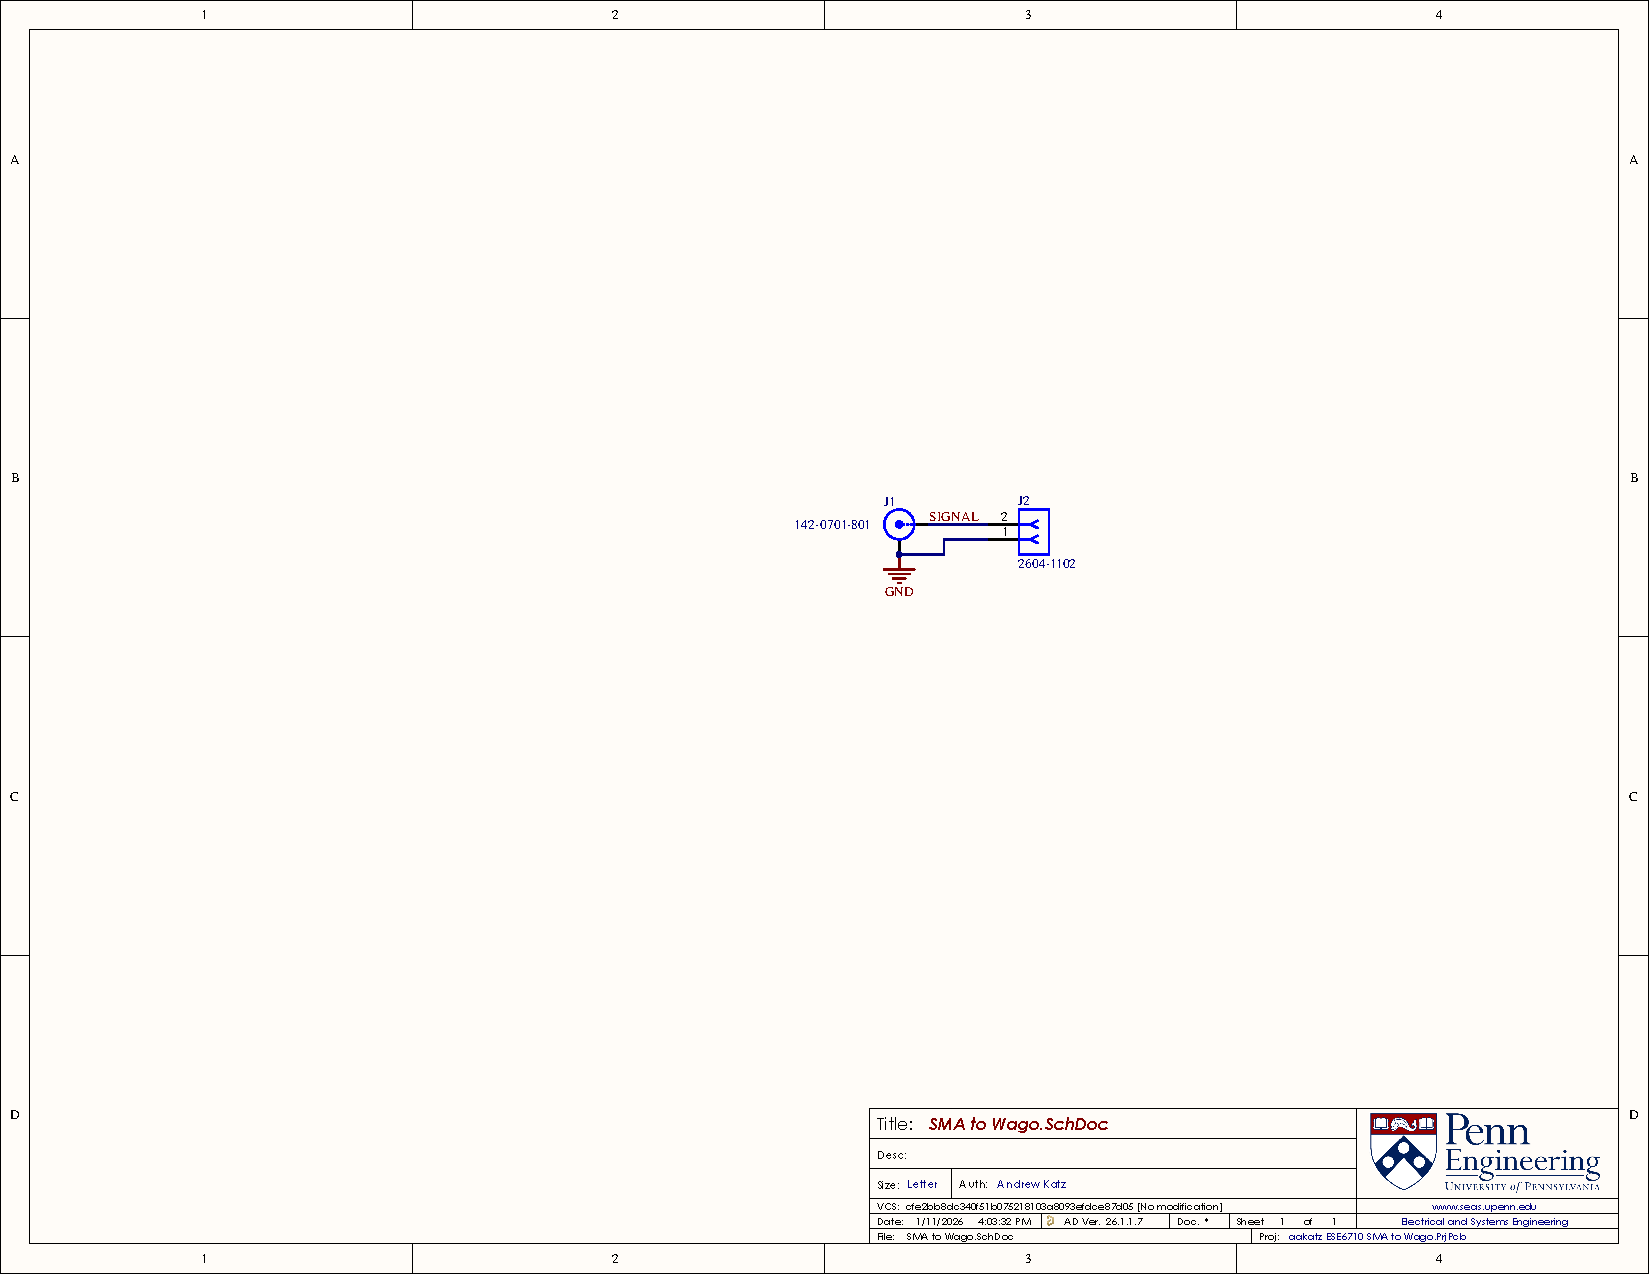
\includegraphics[trim=5.in 4.25in 3.5in 3in, clip, width=0.5\linewidth]{figure/sch/sma_to_wago.pdf}
        \caption{Schematic drawing for the SMA to Wago adapter}
        \label{fig:sch:sma-wago}
    \end{figure}
    \begin{figure}[H]
        \centering
        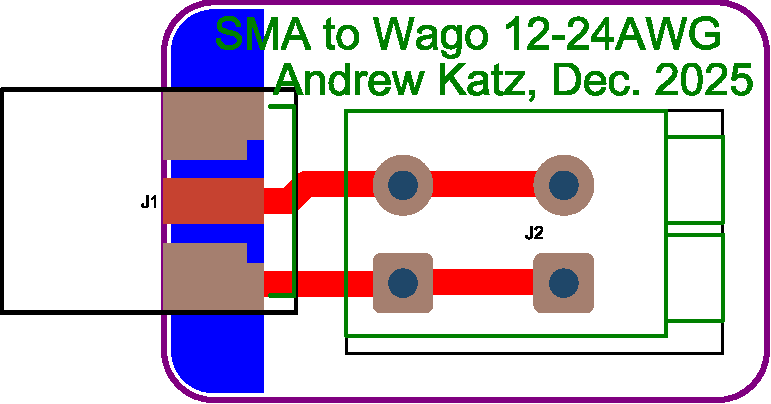
\includegraphics[width=0.4\linewidth]{figure/pcb_layout/sma_to_wago_pcb.pdf}
        \caption{CAD drawing of PCB layout for the SMA to Wago adapter}
        \label{fig:pcb:sma-wago}
    \end{figure}
    \begin{figure}[H]
        \centering
        \subfloat[]{\includegraphics[height=80pt]{figure/photo/board/sma_wago_plug_edit.PNG}\label{fig:board:sma-wago-plug}}
        \hfil
        \subfloat[]{\includegraphics[height=80pt]{figure/photo/board/sma_wago_jack_edit.PNG}\label{fig:board:sma-wago-jack}}
        
        \caption{
            \centering
            Assembled SMA to Wago adapter:\quad
            (a) Plug version
            (b) Jack version
        }
        \label{fig:board_sma-wago}
    \end{figure}
    \begin{table}[H]
        \centering
        % !TeX document-id = {bf507081-e2df-4597-a7a4-c771a1a51ffd}
% !TeX program = pdftex
\documentclass{standalone}
\usepackage{booktabs}
\begin{document}
    \centering
    \begin{tabular}{lcccl}
        \toprule
        \textbf{Name} & \textbf{Designator} &  \textbf{Varient} & \textbf{Manufacturer} & \textbf{Part Number} \\
        \midrule
        CON-SMA-EDGE & J1 & Wide SMA Jack & RF Solutions & CON-SMA-EDGE \\
        EMPCB.SMAMST.A & J1 & SMA Plug & Taoglas & EMPCB.SMAMST.A \\
        2604-1102 & J2 & All & WAGO & 2604-1102 \\
        \bottomrule
    \end{tabular}
\end{document}
        \caption{BOM for the SMA to Wago adapter}
    \end{table}
    %    \FloatBarrier
    \section{Other Content}
    \raggedright
    
    A GitHub repository with all of the code, data, and any relevant instructions can be found at:
    \url{https://github.com/aakatz3/ESE6710-Final-Project}
    
    \section{Equipment Used}
    The following is a list of all measurement equipment utilized in \cref{sec:exp} where results were recorded:
    \begin{itemize}
        \item \href{https://www.keysight.com/us/en/product/E3631A/80w-triple-output-power-supply-6v-5a--25v-1a.html}{Keysight (formerly Agilent/Hewlett--Packard) E3631A Triple Output Power Supply, 6V, 5A \& ±25V, 1A}
        \item \href{https://www.keysight.com/us/en/product/E3634A/200w-power-supply-25v-7a-50v-4a.html}{Keysight (formerly Agilent/Hewlett--Packard) E3634A 200W Power Supply, 25V, 7A or 50V, 4A}
        \item \href{https://www.keysight.com/us/en/product/33521A/function--arbitrary-waveform-generator-30-mhz.html}{Keysight (formerly Agilent) 33521A Function / Arbitrary Waveform Generator, 30 MHz}
        \item \href{https://www.keysight.com/us/en/product/33510B/waveform-generator-20-mhz-2-channel.html}{Keysight 33510B Waveform Generator, 20 MHz, 2--Channel}
        \item \href{https://www.keysight.com/us/en/product/MSO7034B/mixed-signal-oscilloscope-350mhz-4-analog-16-digital-channels.html}{Keysight (formerly Agilent) MSO7034B Mixed Signal Oscilloscope: 350 MHz, 4 Analog plus 16 Digital Channels}
        \item \href{https://www.keysight.com/us/en/product/MSO6014A/mixed-signal-oscilloscope-100-mhz-4-analog-16-digital-channels.html}{Keysight (formerly Agilent) MSO6014A Mixed Signal Oscilloscope: 100 MHz, 4 Analog and 16 Digital Channels}
        \item \href{https://www.keysight.com/us/en/product/N2791A/high-voltage-differential-probe-25-mhz.html}{Keysight N2791A High-Voltage Differential Probe, 25 MHz}
        \item \href{https://www.keysight.com/us/en/product/1147B/ac-dc-current-probe-50-mhz-15a.html}{Keysight 1147B AC/DC Current Probe, 50 MHz, 15A}
        \item \href{https://www.keysight.com/us/en/product/10073D/passive-probe-10-1-500-mhz-1-5-m.html}{Keysight (formerly Agilent) 10073D Passive Probe, 10:1, 500 MHz, 1.5 m}
        \item \href{https://www.keysight.com/us/en/product/N2890A/passive-probe-10-1-500mhz-1-3m.html}{Keysight (formerly Agilent) N2890A Passive Probe, 10:1, 500 MHz, 1.3m}
        \item \href{https://www.keysight.com/us/en/product/N2889A/passive-probe-10-1-1-1-350-mhz-1-3m.html}{Keysight (formerly Agilent) N2889A Passive Probe, 10:1/1:1, 350 MHz, 1.3m}
        \item \href{https://www.keysight.com/us/en/product/34401A/digital-multimeter-6-digit.html}{Keysight (formerly Agilent/Hewlett--Packard) 34401A Digital Multimeter, 6½ Digit}
        \item \href{https://www.keysight.com/us/en/product/EDU34450A/smart-bench-essentials-digital-multimeter-5-5-digit.html}{Keysight EDU34450A Smart Bench Essentials Digital Multimeter}
        \item \href{https://www.keysight.com/us/en/product/EL34143A/dc-electronic-load-single-input-150v-60a-350w-lan-usb.html}{Keysight EL34143A 350W Bench Electronic Load, Single Input 150V, 60A, 350W}
        \item \href{https://www.keysight.com/us/en/product/E4980AL/precision-lcr-meter-20-hz-300-khz-500-khz-1-mhz.html}{Keysight E4980AL Precision LCR Meter 20 Hz to 300 kHz / 500 kHz / 1 MHz}
        \item \href{https://www.keysight.com/us/en/product/E5063A/e5063a-ena-vector-network-analyzer.html}{Keysight (formerly Agilent) E5063A ENA Vector Network Analyzer}
        \item \href{https://www.keysight.com/us/en/product/N7554A/electronic-calibration-module-ecal-dc-18-ghz-2-port.html}{Keysight N7554A Electronic Calibration Module (ECal), DC-18 GHz, 2-Port}
        \item \href{https://www.rohde-schwarz.com/us/products/test-and-measurement/benchtop-analyzers/rs-fpc-spectrum-analyzer_63493-542324.html}{Rohde \& Schwarz FPC1000}
        \item \href{https://www.minicircuits.com/WebStore/dashboard.html?model=ZFL-1000LNB%2B}{Mini-Circuits ZFL-1000LNB+ Connectorized SMA, Low Noise, Linear Amplifier, 0.1 MHz to 1000 MHz, 50Ω}
        \item \href{https://www.yageogroup.com/products/Resistors/part/RC1206FR-131ML}{Yageo 1 MOhms ±1\% 0.25W, 1/4W Chip Resistor 1206 (3216 Metric) Moisture Resistant Thick Film}
        \item \href{https://www.amazon.com/40dB-Attenuator-Precision-Adjustable-Communication/dp/B0F9VRD3KJ}{BECEN 200W N-Type 40dB Attenuator, DC to 3GHz, 50 Ohms, Precision Adjustable Signal Loss for RF Systems, Testing, Broadcast \& Communication}
        \item \href{https://www.l-com.com/bandpass-filter-rf-splitter-0-6-ghz-type-n-male-terminator-50-ohm}{L-com 0-6 GHz Type N Male Terminator 50 Ohm}
    \end{itemize}
\end{appendices}